%% =====================================================================
%%  PGARA: Profile-Guided Adaptive Register Allocation
%%  IEEE conference manuscript (IEEEtran).  Compile with:
%%      pdflatex pgara && pdflatex pgara
%%  External files are the GUI screenshots gui_*.png; the manuscript still
%%  compiles (with framed boxes in their place) if they are missing.
%% =====================================================================
\documentclass[conference]{IEEEtran}
\IEEEoverridecommandlockouts

\usepackage{cite}
\usepackage{amsmath,amssymb,amsfonts}
\usepackage{stmaryrd}
\usepackage{algorithm}
\usepackage{algorithmic}
\usepackage{graphicx}
\usepackage{textcomp}
\usepackage{xcolor}
\usepackage{booktabs}
\usepackage{multirow}
\usepackage{array}
\usepackage{url}
\usepackage{tikz}
\usetikzlibrary{arrows.meta,positioning,shapes.geometric,fit,calc,backgrounds}
\usepackage{pgfplots}
\pgfplotsset{compat=1.18}

\definecolor{ink}{HTML}{111827}
\definecolor{card}{HTML}{F3F4F6}
\definecolor{rule}{HTML}{E5E7EB}
\definecolor{mid}{HTML}{6B7280}
\definecolor{indigo}{HTML}{4F46E5}
\definecolor{violet}{HTML}{7C3AED}
\definecolor{emerald}{HTML}{059669}
\definecolor{amber}{HTML}{D97706}
\definecolor{orangeC}{HTML}{EA580C}
\definecolor{rose}{HTML}{DB2777}
\definecolor{sky}{HTML}{0284C7}
\definecolor{redC}{HTML}{DC2626}
\definecolor{slate}{HTML}{64748B}
\definecolor{cPG}{HTML}{6366F1}
\definecolor{cSP}{HTML}{0EA5E9}
\definecolor{cLD}{HTML}{F59E0B}
\definecolor{cLS}{HTML}{64748B}

\newtheorem{definition}{Definition}
\newtheorem{proposition}{Proposition}
\newenvironment{proofsketch}{\noindent\textit{Proof sketch.}\ }{\hfill$\square$\par}

\newcommand{\MG}{PGARA}
\newcommand{\Reg}{\mathsf{R}}
\newcommand{\Mem}{\mathsf{M}}
\newcommand{\cld}{c_{\mathrm{ld}}}
\newcommand{\cst}{c_{\mathrm{st}}}
\newcommand{\csv}{\sigma}
\newcommand{\cmv}{c_{\mathrm{mv}}}
\newcommand{\First}{\mathrm{FIRST}}
\newcommand{\Follow}{\mathrm{FOLLOW}}
\newcommand{\nt}[1]{\textit{#1}}
\newcommand{\tm}[1]{\texttt{#1}}

\tikzset{
  stage/.style={draw=sky, rounded corners=2pt, fill=sky!8, align=center, line width=0.6pt,
                font=\scriptsize, minimum height=7.5mm, inner sep=2pt},
  midst/.style={stage, draw=emerald, fill=emerald!9},
  hot/.style={stage, draw=indigo, top color=indigo, bottom color=violet, text=white},
  back/.style={stage, draw=amber, fill=amber!10},
  flow/.style={-{Stealth[length=1.6mm]}, draw=ink!80, line width=0.55pt},
  soft/.style={-{Stealth[length=1.4mm]}, draw=violet!70, dashed, line width=0.5pt},
  blk/.style={draw=slate, rounded corners=1.5pt, fill=white, align=left,
              font=\scriptsize\ttfamily, inner sep=2.5pt},
}

\begin{document}

\title{PGARA: Profile-Guided Adaptive Register Allocation\\[2pt]
\large Stochastic Dynamic Programming and Game-Theoretic Auctions in an
End-to-End Compiler, Without Graph Colouring}

\author{
\IEEEauthorblockN{Shreyans Chowdry}
\IEEEauthorblockA{Reg.\ No.\ 24BDS0114\\
Vellore Institute of Technology\\Vellore, India}
\and
\IEEEauthorblockN{Samrender Singh Saini}
\IEEEauthorblockA{Reg.\ No.\ 24BCE2865\\
Vellore Institute of Technology\\Vellore, India}
\and
\IEEEauthorblockN{Karthikeya Jami}
\IEEEauthorblockA{Reg.\ No.\ 24BCE2136\\
Vellore Institute of Technology\\Vellore, India}
\and
\IEEEauthorblockN{Abhishek Kumar}
\IEEEauthorblockA{Reg.\ No.\ 24BCE0585\\
Vellore Institute of Technology\\Vellore, India}
\and
\IEEEauthorblockN{Nishanth Kumar}
\IEEEauthorblockA{Reg.\ No.\ 24BAI0194\\
Vellore Institute of Technology\\Vellore, India}
}

\maketitle

%% ---------------------------------------------------------------------
\begin{abstract}
Optimising compilers translate high-level programs into machine code
for processors with only a handful of fast registers, and the register
allocator, which decides which values live in those registers, is one of
the largest single contributors to the quality of the generated code.
The allocator has to decide, for every value, whether to keep it in a
register or spill it to memory, and the right answer depends on how
often each path through the program is actually taken, which the
compiler does not know statically.
Production allocators colour an interference graph or scan live
intervals, ranking spill candidates by static use counts or
$10^{\text{loop depth}}$ weights; recent learned allocators train neural
policies on large corpora.
Static weights are blind to data-dependent branches, and learned
policies are costly to train and offer no per-decision explanation.
We present PGARA (Profile-Guided Adaptive Register Allocation), which
adapts every register decision to the program's measured behaviour. It
models the residency of every SSA value as a
two-state Markov decision process over the control-flow graph, with
transition probabilities measured by profiling. Exact policy iteration
yields each value's expected register-residency gain, values sharing a
loop-carried $\varphi$-web bid as one coalition, and registers are sold
in a sealed-bid auction along a maximum-cardinality-search order of the
chordal SSA interference graph, refined by best-response dynamics to a
pure Nash equilibrium. \MG\ is embedded in a complete compiler for a
C subset (DFA lexer, LL(1) parser, attribute-grammar semantic analysis,
three-address code, SSA optimiser, PG-RISC code generator and
cycle-counting simulator) with a web interface that visualises every phase.
Across ten benchmarks and five register budgets, all 200 compiled
programs produce reference-identical output; at $k{=}4$ registers \MG\
lowers the geometric-mean cycle count by 20.5\% relative to linear scan,
6.4\% relative to loop-depth priority and 2.5\% relative to the same
engine driven by static branch priors, and cuts dynamic spill traffic
by 59\% relative to linear scan.
Future work will add live-range splitting to the MDP and evaluate the
allocator inside a production back end on standard suites.
\end{abstract}

\begin{IEEEkeywords}
Compiler design, game theory, Markov decision process,
profile-guided optimization, register allocation, static single assignment
\end{IEEEkeywords}

%% =====================================================================
\section{Introduction}
\label{sec:intro}

Compilers are the bridge between the abstractions programmers write and
the narrow interface that hardware executes. Their structure has been
stable for decades (a front end that recognises and checks the
language, a middle end that transforms a machine-independent
intermediate representation, and a back end that maps it to
instructions and registers), but the techniques inside each phase keep
evolving, from reusable multi-level infrastructures such as
MLIR~\cite{lattner2021mlir} to optimisation heuristics learned from
data~\cite{wang2018ml,ashouri2018survey,leather2020ml}. Static single
assignment (SSA) form~\cite{cytron1991ssa,rastello2022ssa} is now the
common currency of this middle end, and the textbooks used to teach the
subject treat it as such~\cite{cooper2022eac,aho2006dragon}.

Among back-end problems, register allocation has an outsized effect on
performance: a value that is not kept in a register costs a store when
it is produced and a load each time it is consumed, and on a loop that
runs millions of times these accesses dominate execution time. The
problem is hard for two reasons. First, the decision is combinatorial,
since values that are live at the same time compete for the same $k$
registers. Second, the payoff of each decision is uncertain at compile
time, because it depends on which branches the program actually takes.
A value used only on an error path that runs once in a thousand
iterations is worth far less than one used on the hot path, yet a
static analysis sees the two paths as symmetric. Our motivation is to
treat this second difficulty as a first-class modelling concern rather
than a tuning detail.

Existing allocators fall broadly into three families. Graph-colouring
allocators, descending from Chaitin~\cite{chaitin1982} and the
priority-based variant of Chow and Hennessy~\cite{chow1990}, build an
interference graph and colour it with $k$ colours, choosing spill
candidates by a cost that weights each access by $10^{d}$ for loop depth
$d$. Linear-scan allocators~\cite{poletto1999} trade quality for speed
by sweeping live intervals in program order. On SSA form the
interference graph is chordal~\cite{hack2006ssa,hack2006ipl}, which makes
colouring itself polynomial and moves the difficulty entirely into the
spilling decision; combinatorial approaches solve allocation and
scheduling jointly to proven optimality~\cite{lozano2019toplas,lozano2019survey}.

A newer family learns allocation and related decisions from data.
MLGO~\cite{trofin2021mlgo} trains policies inside LLVM's production
allocator, RL4ReAl~\cite{venkatakeerthy2023rl4real} learns end-to-end
register allocation with reinforcement learning over embeddings such as
IR2Vec~\cite{venkatakeerthy2020ir2vec}, and environments such as
CompilerGym~\cite{cummins2022compilergym} and representations such as
ProGraML~\cite{cummins2021programl} make these experiments
reproducible. In parallel, profile-guided post-link optimisers such as
BOLT~\cite{panchenko2019bolt} and Propeller~\cite{shen2023propeller}
have shown that measured execution profiles yield large gains in code
layout, and recent work predicts profiles when none are
available~\cite{rotem2021pgo}.

These families leave a gap. Static spill weights encode a fixed belief
about branch behaviour (loops iterate about ten times; both arms of a
conditional are equally likely), so they mis-rank values precisely on
programs with data-dependent control flow, as early studies of static
estimators already observed~\cite{wagner1994,wu1994}. Learned policies
avoid fixed beliefs, but they require large training corpora and
expensive training loops~\cite{sutton2018rl}, and the decision they make
for a particular value cannot be traced back to a quantity a compiler
engineer can inspect.

Classical colouring formulations also obscure the objective. A
colouring is either feasible or not, and the quality of the result
emerges indirectly from the order in which nodes are simplified and
spilled. Neither family states, for each value, the expected number of
cycles that keeping it in a register will save.

We propose \MG\ (Profile-Guided Adaptive Register Allocation), which
makes that expected saving the central quantity. It is profile-guided
because every probability it uses is measured on a training run, and
adaptive because the same program receives a different allocation when
its measured behaviour changes, without any hand-tuned weights.
Each SSA value's residency is a two-state Markov decision process (MDP)
over its live range in the control-flow graph~\cite{puterman1994,bertsekas2019};
transition probabilities are measured edge frequencies, and exact policy
iteration~\cite{howard1960} gives the value's expected gain per
invocation. Allocation is then a resource-contention game: values that
form a loop-carried $\varphi$-web bid together as a coalition, in the
spirit of cooperative game theory~\cite{shapley1953}, registers are sold
in a sealed-bid auction~\cite{vickrey1961} processed along a
maximum-cardinality-search (MCS) order~\cite{tarjan1984} of the chordal
interference graph, and best-response dynamics settle the result into a
pure Nash equilibrium~\cite{rosenthal1973,nisan2007agt}. The approach
is apt because each ingredient matches a structural fact of the problem:
SSA makes the contention structure chordal, profiles make the
uncertainty measurable, and the gain is an explicit, inspectable number.

The advantages are practical as well as conceptual. Policy iteration on
a two-state MDP per value converges in about 1.3 improvement rounds on
average, so allocation takes milliseconds; every decision can be
explained by a bid and an auction round; and the same engine runs
unchanged on static priors, which isolates the value of profiling.
To evaluate it honestly we built a complete compiler around it, from a
formally specified grammar to a cycle-counting simulator, and a web
interface that renders every intermediate artefact.

The remainder of the paper is organised as follows.
Section~\ref{sec:related} reviews fifteen recent works and the gaps they
leave. Section~\ref{sec:proposed} formalises the language, the front
end, the intermediate representations and the optimiser, then develops
the MDP, the gain, the coalitions and the auction, with the algorithms
and their properties. Section~\ref{sec:impl} describes the toolchain,
the parameters and the results on five metrics against three baselines.
Section~\ref{sec:conclusion} concludes, and the team's contributions are
listed after it.

%% =====================================================================
\section{Related Works}
\label{sec:related}

We review fifteen works from 2018--2024, grouped by theme. For each we
summarise the proposed solution, its methodology and tools, the reported
effectiveness and the research gap relative to \MG.

\subsection{Combinatorial and survey work on allocation}

\textit{Castañeda Lozano et~al.}~\cite{lozano2019toplas} propose Unison,
which formulates global register allocation (including spilling,
coalescing and live-range splitting) together with instruction
scheduling as a single constraint model. Programs are first transformed
into linear SSA, the model is solved with a constraint programming
solver using problem-specific decomposition, and it is integrated with
LLVM for Hexagon, ARM and MIPS. Unison produces provably optimal or
near-optimal code for functions of up to about a thousand instructions
and improves on LLVM's heuristics for a measurable fraction of them.
\textit{Gap:} the objective is a static cost estimate, and solve times
grow quickly with function size.

\textit{Castañeda Lozano and Schulte}~\cite{lozano2019survey} survey
combinatorial approaches to register allocation and instruction
scheduling. They classify integer programming, constraint programming,
PBQP and related models by the subproblems covered, by scalability and
by the quality of the code produced, and compare reported evaluations
across targets. The survey shows that combinatorial methods reach
optimality on medium-sized functions but are seldom used in production.
\textit{Gap:} almost all surveyed models assume static frequency
estimates rather than measured, stochastic behaviour.

\subsection{Learning-based allocation and program representation}

\textit{VenkataKeerthy et~al.}~\cite{venkatakeerthy2023rl4real} present
RL4ReAl, a reinforcement-learning register allocator. The interference
graph is embedded with IR2Vec features and a hierarchy of agents learns
to pick nodes to colour, spill or split, trained with policy-gradient
methods inside an LLVM-based gRPC environment for x86 and AArch64. The
learned allocator matches or improves on LLVM's greedy allocator on
several benchmark suites. \textit{Gap:} training is costly and
individual decisions are not interpretable as expected savings.

\textit{Trofin et~al.}~\cite{trofin2021mlgo} introduce MLGO, a framework
for integrating trained policies in LLVM. Policies for inlining-for-size
and, later, register-allocation eviction are trained offline with
reinforcement learning and evolution strategies on corpora of production
code and shipped as compiled TensorFlow models. Inlining-for-size
achieved several percent size reduction on large binaries.
\textit{Gap:} policies generalise from a corpus, not from the profile of
the program being compiled.

\textit{Cummins et~al.}~\cite{cummins2022compilergym} present
CompilerGym, a set of environments that expose compiler optimisation
problems through the OpenAI Gym interface. It wraps LLVM phase ordering,
GCC flag tuning and loop-nest generation behind a client-server
architecture, with datasets of millions of programs and multiple
observation spaces. It made reinforcement-learning experiments on
compilers reproducible and fast. \textit{Gap:} it targets pass-level
decisions, not per-value register decisions.

\textit{Cummins et~al.}~\cite{cummins2021programl} propose ProGraML, a
graph representation of programs that combines control, data and call
flow, processed by gated graph neural networks. The representation is
built from LLVM and XLA IR and evaluated on data-flow analyses and
heuristics such as device mapping and thread coarsening. It
outperformed sequence-based representations on those tasks.
\textit{Gap:} it learns to approximate analyses that \MG\ computes
exactly.

\textit{VenkataKeerthy et~al.}~\cite{venkatakeerthy2020ir2vec} introduce
IR2Vec, distributed embeddings of LLVM IR derived from a learned
seed-embedding vocabulary and flow analysis. Embeddings are computed at
instruction, function and program level without heavy training, and used
for heterogeneous device mapping and thread-coarsening prediction with
competitive accuracy. \textit{Gap:} embeddings capture syntax and flow,
not execution frequencies.

\textit{Jain et~al.}~\cite{jain2022posetrl} propose POSET-RL, which
orders optimisation passes with reinforcement learning. A partially
ordered set of pass sub-sequences derived from LLVM's O-levels defines
the action space, and a deep Q-network trained on IR2Vec states optimises
size and execution time. It reduced code size and runtime relative to
the standard pipeline on SPEC and MiBench. \textit{Gap:} it operates
above the allocator and treats it as a black box.

\textit{Haj-Ali et~al.}~\cite{hajali2020neurovectorizer} present
NeuroVectorizer, which learns vectorisation and interleaving factors
with deep reinforcement learning. Loops are embedded with code2vec and a
policy chooses pragmas that Clang/LLVM applies, with rewards measured by
execution time. It outperformed the baseline cost model on a range of
loop kernels. \textit{Gap:} measured rewards drive training, but the
decision is not grounded in a model of the program's behaviour.

\subsection{Surveys of machine learning in compilers}

\textit{Wang and O'Boyle}~\cite{wang2018ml} survey machine learning in
compiler optimisation. They organise the field by feature engineering,
learning models and deployment, covering search-based tuning,
predictive modelling and deep learning across many published systems,
and show consistent gains over hand-written heuristics.
\textit{Gap:} register allocation is barely represented, and the role of
measured profiles inside heuristics is left open.

\textit{Ashouri et~al.}~\cite{ashouri2018survey} survey compiler
autotuning with machine learning, with an emphasis on optimisation
selection and phase ordering. They classify works by learning model,
features and prediction type and summarise the tools used, from
Milepost-GCC to LLVM-based frameworks, reporting the speed-ups achieved.
\textit{Gap:} the focus is on choosing passes, not on resource
assignment inside a pass.

\subsection{Profile-guided optimisation}

\textit{Panchenko et~al.}~\cite{panchenko2019bolt} present BOLT, a
post-link optimiser that uses sampled hardware profiles. It rewrites
binaries using LLVM's MC infrastructure and reorders basic blocks and
functions according to Linux \texttt{perf} profiles collected in
production. It gave substantial speed-ups on large data-centre
applications already built with feedback-directed optimisation.
\textit{Gap:} it uses profiles for layout only; register decisions are
fixed before it runs.

\textit{Shen et~al.}~\cite{shen2023propeller} present Propeller, a
profile-guided relinking optimiser for warehouse-scale applications. It
integrates profile-driven basic-block layout into the build through
distributed, incremental relinking with the LLVM toolchain, avoiding
BOLT's monolithic binary rewrite. It achieved comparable speed-ups with
much lower memory and build-time cost. \textit{Gap:} as with BOLT, the
profile does not reach allocation.

\textit{Rotem and Cummins}~\cite{rotem2021pgo} predict branch
probabilities statically so that profile-guided optimisation can run
without profiles. A gradient-boosted model is trained on features of
branches in a large corpus of profiled code and its predictions are fed
into LLVM's PGO pipeline. A substantial share of the benefit of real
profiles was recovered. \textit{Gap:} predicted probabilities feed
existing static heuristics rather than an allocation model that uses
them directly.

\subsection{Infrastructure and large language models}

\textit{Lattner et~al.}~\cite{lattner2021mlir} introduce MLIR, a
multi-level compiler infrastructure with extensible dialects, regions
and SSA-based IR that is shared across domains. It is implemented in
C++ within the LLVM project and used to build compilers for machine
learning, hardware design and more. It reduced the cost of building
domain-specific compilers. \textit{Gap:} MLIR lowers to LLVM's
allocators and does not change how registers are assigned.

\textit{Cummins et~al.}~\cite{cummins2023llm} train a large language
model to optimise LLVM assembly for code size. A 7B-parameter
transformer is trained from scratch to predict pass lists and optimised
IR, with auxiliary tasks that improve its understanding of the code.
It outperformed the compiler's built-in pass ordering on held-out
programs with no extra compilations. \textit{Gap:} its outputs are not
guaranteed correct and give no account of the decisions made.

\subsection{Summary of gaps}

Across these works, measured execution frequencies drive layout but not
allocation, learned allocators require heavy training and are opaque,
and combinatorial allocators optimise static cost models. \MG\
addresses the intersection: an allocator whose objective is the
expected saving under measured probabilities, solved exactly and
cheaply, with every decision explainable as a bid.

%% =====================================================================
\section{Proposed Work}
\label{sec:proposed}

\subsection{Problem formulation}

Let a function in SSA form have values $V$, a control-flow graph (CFG)
$\mathcal{C}=(B,E,b_0)$ and a register file of $k$ registers. An
allocation is a map $\rho: V \to \{0,\dots,k{-}1\}\cup\{\bot\}$ in which
$\rho(v)=\bot$ means that $v$ lives in its stack slot; it is feasible
when no two interfering values share a register. Executing the program
on an input induces a random walk over $\mathcal{C}$, and the cost of
the allocation is the expected number of cycles spent on loads, stores
and copies caused by values without a register. We seek
\begin{equation}
\rho^\star \;=\; \arg\max_{\rho\ \text{feasible}}\;
\sum_{v:\,\rho(v)\neq\bot} G(v),
\label{eq:objective}
\end{equation}
where $G(v)$ is the expected cycles saved by giving $v$ a register,
computed under transition probabilities measured by profiling.

Two features make (\ref{eq:objective}) tractable without colouring.
On strict SSA form the interference graph is chordal~\cite{hack2006ssa},
so the values competing at any program point form a clique that an MCS
order exposes one at a time. And the gain of a single value can be
computed exactly by stochastic dynamic programming over its live range,
because the residency of one value is a small MDP whose only uncertainty
is the branch behaviour of the CFG. Both observations are developed
below, after the front end and middle end that produce the SSA program.

\subsection{System architecture}

Fig.~\ref{fig:arch} shows the architecture. The front end turns MiniC
source text into a type-checked abstract syntax tree (AST) and symbol
table; the middle end lowers it to three-address code (TAC), builds the
CFG, constructs SSA and optimises it; a reference interpreter executes
the optimised SSA on a training input and records edge counts; the
\MG\ engine converts those counts into gains, coalitions and an
auctioned allocation; and the back end leaves SSA, emits PG-RISC code
and runs it on a cycle-counting simulator on a separate test input.

Every stage reports its result into a single JSON document, which the
web interface renders as token streams, AST, symbol tables, TAC, SSA,
CFG, interference graph, auction rounds and target code (dashed arrows
in Fig.~\ref{fig:arch}). Three baseline allocators share the same
pipeline and code generator, so differences in the measured cycles
are attributable to allocation decisions alone.

\begin{figure*}[!t]
\centering
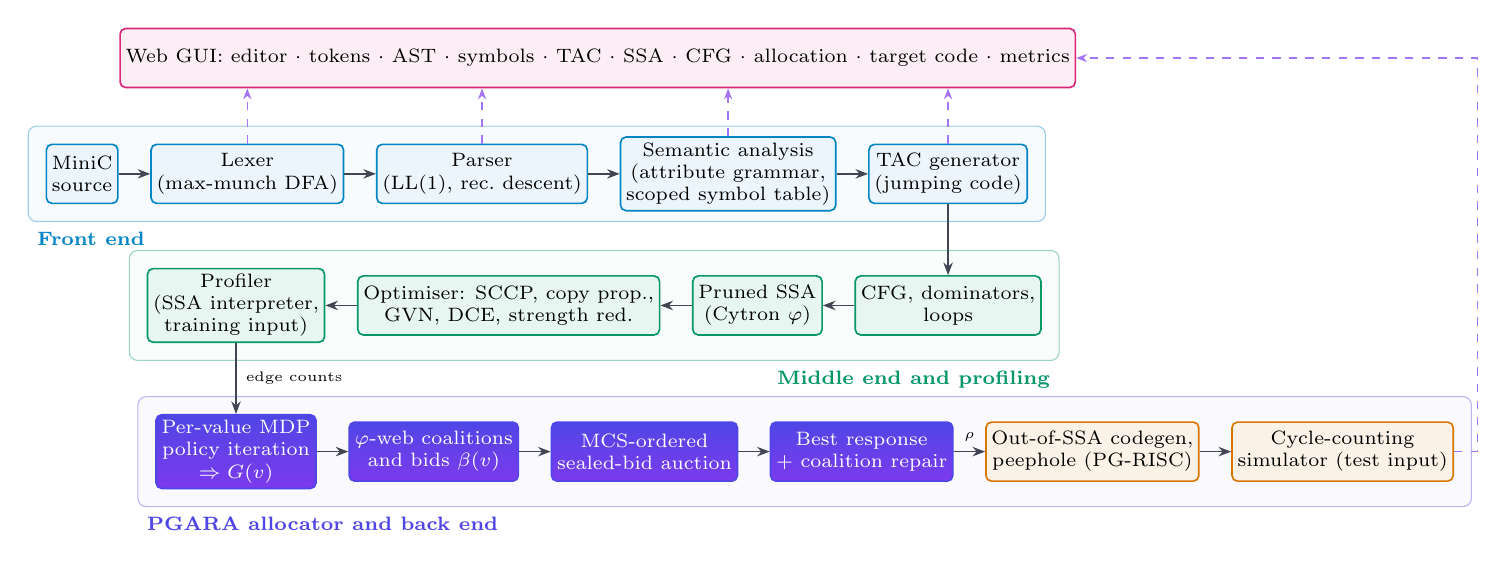
\begin{tikzpicture}[node distance=4.5mm and 4mm]
  % Front end
  \node[stage] (src) {MiniC\\source};
  \node[stage, right=of src] (lex) {Lexer\\(max-munch DFA)};
  \node[stage, right=of lex] (par) {Parser\\(LL(1), rec.\ descent)};
  \node[stage, right=of par] (sem) {Semantic analysis\\(attribute grammar,\\scoped symbol table)};
  \node[stage, right=of sem] (tac) {TAC generator\\(jumping code)};
  % Middle end
  \node[midst, below=9mm of tac] (cfg) {CFG, dominators,\\loops};
  \node[midst, left=of cfg] (ssa) {Pruned SSA\\(Cytron $\varphi$)};
  \node[midst, left=of ssa] (opt) {Optimiser: SCCP, copy prop.,\\GVN, DCE, strength red.};
  \node[midst, left=of opt] (prof) {Profiler\\(SSA interpreter,\\training input)};
  % PGARA allocator
  \node[hot, below=9mm of prof] (mdp) {Per-value MDP\\policy iteration\\$\Rightarrow G(v)$};
  \node[hot, right=of mdp] (coal) {$\varphi$-web coalitions\\and bids $\beta(v)$};
  \node[hot, right=of coal] (auc) {MCS-ordered\\sealed-bid auction};
  \node[hot, right=of auc] (br) {Best response\\+ coalition repair};
  \node[back, right=of br] (cg) {Out-of-SSA codegen,\\peephole (PG-RISC)};
  \node[back, right=of cg] (sim) {Cycle-counting\\simulator (test input)};
  % GUI
  \node[stage, draw=rose, fill=rose!8, above=7mm of $(lex.north)!0.5!(tac.north)$, minimum width=95mm] (gui)
       {Web GUI: editor $\cdot$ tokens $\cdot$ AST $\cdot$ symbols $\cdot$ TAC $\cdot$ SSA $\cdot$ CFG $\cdot$ allocation $\cdot$ target code $\cdot$ metrics};
  \draw[flow] (src) -- (lex);
  \draw[flow] (lex) -- (par);
  \draw[flow] (par) -- (sem);
  \draw[flow] (sem) -- (tac);
  \draw[flow] (tac) -- (cfg);
  \draw[flow] (cfg) -- (ssa);
  \draw[flow] (ssa) -- (opt);
  \draw[flow] (opt) -- (prof);
  \draw[flow] (prof) -- node[right,font=\tiny]{edge counts} (mdp);
  \draw[flow] (mdp) -- (coal);
  \draw[flow] (coal) -- (auc);
  \draw[flow] (auc) -- (br);
  \draw[flow] (br) -- node[above,font=\tiny]{$\rho$} (cg);
  \draw[flow] (cg) -- (sim);
  \draw[soft] (sem.north) -- (sem.north |- gui.south);
  \draw[soft] (par.north) -- (par.north |- gui.south);
  \draw[soft] (lex.north) -- (lex.north |- gui.south);
  \draw[soft] (tac.north) -- (tac.north |- gui.south);
  \draw[soft] (sim.east) -- ++(3mm,0) |- (gui.east);
  \begin{scope}[on background layer]
    \node[draw=sky!40, fill=sky!3, rounded corners=3pt, inner sep=2.2mm,
          fit=(src)(tac), label={[font=\scriptsize\bfseries,text=sky,anchor=north west]south west:Front end}] {};
    \node[draw=emerald!40, fill=emerald!3, rounded corners=3pt, inner sep=2.2mm,
          fit=(prof)(cfg), label={[font=\scriptsize\bfseries,text=emerald,anchor=north east]south east:Middle end and profiling}] {};
    \node[draw=indigo!40, fill=indigo!3, rounded corners=3pt, inner sep=2.2mm,
          fit=(mdp)(sim), label={[font=\scriptsize\bfseries,text=indigo,anchor=north west]south west:\MG\ allocator and back end}] {};
  \end{scope}
\end{tikzpicture}
\caption{Architecture of the \MG\ compiler: front end (blue), middle
end and profiling (green), the \MG\ allocation engine (indigo) and back
end (amber). Dashed violet arrows show phase reports consumed by the web
interface (pink).}
\label{fig:arch}
\end{figure*}

\subsection{Front end: language, grammar and parsing}

\paragraph*{Lexical analysis}
MiniC has \tm{int} scalars and one-dimensional arrays, array parameters
passed by reference, functions, \tm{if}/\tm{else}, \tm{while},
\tm{for}, \tm{break}, \tm{continue}, \tm{print} and \tm{input()}, the
arithmetic, relational and short-circuit logical operators, and the
compound forms \tm{+=}, \tm{-=}, \tm{*=}, \tm{++}, \tm{--}. The lexer is
a deterministic finite automaton applied under the maximal-munch rule:
from position $i$ it returns the longest prefix $w$ of the remaining
input with $\delta^\ast(q_0,w)\in F$, so \tm{<=} is one token and
\tm{a+++b} is \tm{a ++ + b}. Keywords are recognised as identifiers and
reclassified by table lookup. An invalid character is reported with its
line and column and skipped (panic mode), so later errors are still
found in the same run.

\paragraph*{Context-free grammar}
The syntax is the context-free grammar
\begin{equation}
G=(N,\Sigma,P,S),\quad |N|=41,\ |P|=94,\ S=\nt{Program},
\label{eq:grammar}
\end{equation}
written directly in LL(1) form. Left recursion is removed by the
standard tail transformation and precedence is encoded by one
nonterminal per level, for example
\begin{align*}
\nt{Add} &\to \nt{Mul}\ \nt{AddRest}\\
\nt{AddRest} &\to \tm{+}\ \nt{Mul}\ \nt{AddRest} \mid
                \tm{-}\ \nt{Mul}\ \nt{AddRest} \mid \varepsilon\\
\nt{Stmt} &\to \tm{if (}\ \nt{Expr}\ \tm{)}\ \nt{Stmt}\ \nt{ElsePart}\\
          &\phantom{{}\to{}} \mid \tm{while (}\ \nt{Expr}\ \tm{)}\ \nt{Stmt} \mid \cdots\\
\nt{ElsePart} &\to \tm{else}\ \nt{Stmt} \mid \varepsilon .
\end{align*}
The precedence chain, from loosest to tightest binding, is
\nt{Or}, \nt{And}, \nt{Eq}, \nt{Rel}, \nt{Add}, \nt{Mul}, \nt{Unary},
\nt{Primary}, giving the usual C precedence and left associativity.

\paragraph*{FIRST, FOLLOW and the LL(1) property}
For $\alpha\in(N\cup\Sigma)^\ast$ and $A\in N$,
\begin{equation}
\begin{aligned}
\First(\alpha) &= \{a\in\Sigma \mid \alpha \Rightarrow^\ast a\beta\}
                  \cup \{\varepsilon \mid \alpha\Rightarrow^\ast\varepsilon\},\\
\Follow(A) &= \{a\in\Sigma\cup\{\$\} \mid S\$ \Rightarrow^\ast \beta A a \gamma\}.
\end{aligned}
\label{eq:firstfollow}
\end{equation}
Both are computed as least fixpoints of the usual inclusion constraints.
$G$ is LL(1) iff for every pair of alternatives $A\to\alpha\mid\beta$
\begin{equation}
\First\big(\alpha\,\Follow(A)\big)\cap\First\big(\beta\,\Follow(A)\big)=\emptyset .
\label{eq:ll1}
\end{equation}
The toolchain computes (\ref{eq:firstfollow}), builds the predictive
table and checks (\ref{eq:ll1}) mechanically. The single conflict is
the cell (\nt{ElsePart}, \tm{else}): \tm{else} is in $\First(\tm{else}\
\nt{Stmt})$ and, because \nt{ElsePart} can end a \nt{Stmt}, also in
$\Follow(\nt{ElsePart})$. This is the dangling-else ambiguity, resolved
by preferring $\nt{ElsePart}\to\tm{else}\ \nt{Stmt}$ so that an
\tm{else} binds to the nearest unmatched \tm{if}. Every other cell holds
at most one production, so $G$ is LL(1) modulo this resolution.

\paragraph*{Relation to LR parsing}
Every LL(1) grammar is also LR(1)~\cite{knuth1965lr,lewis1968}, so an
LR(1) or LALR parser generator would accept $G$ unchanged apart from the
same dangling-else conflict, which appears there as a shift/reduce
conflict on \tm{else} and is conventionally resolved in favour of
shift, binding \tm{else} the same way. We chose top-down predictive
parsing because a recursive-descent parser is a direct transcription of
the grammar (one procedure per nonterminal), errors can be reported in
terms of the construct being parsed, and the GUI can show the
predictive table, which students can check against
(\ref{eq:firstfollow})--(\ref{eq:ll1}). The parser recovers from syntax
errors in panic mode, discarding tokens until one in the FOLLOW set of
the current construct (for statements, \tm{;} or \tm{\}}) is found.

\subsection{Semantic analysis as an attribute grammar}

Semantic analysis is specified as an L-attributed grammar~\cite{knuth1968attr}
and implemented as a traversal of the AST. Each node carries an
inherited environment $\Gamma$ (a stack of scopes, each a hash map from
names to symbols) and a synthesised type
$\tau\in\{\tm{int},\tm{int[]},\tm{void}\}$. Typical rules are
\begin{equation}
\begin{aligned}
&\nt{Add}\to\nt{Mul}\ \nt{AddRest}:\\
&\quad \nt{AddRest}.\mathit{in}=\nt{Mul}.\mathit{node},\ \
       \nt{Add}.\mathit{node}=\nt{AddRest}.\mathit{out}\\
&\nt{AddRest}\to\tm{+}\ \nt{Mul}\ \nt{AddRest}_1:\\
&\quad \nt{AddRest}_1.\mathit{in}=\mathrm{Bin}(\tm{+},\nt{AddRest}.\mathit{in},\nt{Mul}.\mathit{node}),\\
&\quad \nt{AddRest}.\mathit{out}=\nt{AddRest}_1.\mathit{out}\\
&\nt{AddRest}\to\varepsilon:\quad \nt{AddRest}.\mathit{out}=\nt{AddRest}.\mathit{in}\\
&E\to E_1\ \mathit{op}\ E_2:\quad E.\tau=\tm{int}\ \text{iff}\ E_1.\tau=E_2.\tau=\tm{int}\\
&\nt{Primary}\to\tm{ID}:\quad \nt{Primary}.\tau=\Gamma(\tm{ID}).\tau\ \text{(error if unbound)}
\end{aligned}
\label{eq:attr}
\end{equation}
The inherited attribute $\mathit{in}$ restores left associativity that
the LL(1) transformation removed from the syntax. Fig.~\ref{fig:ast}
shows the flow of attributes on a small statement. Declarations
extend $\Gamma$ in the innermost scope and reject redeclaration in the
same scope; uses resolve outward through enclosing scopes. Functions
are collected in a first pass, so calls may precede definitions. The
analyser checks arity and argument kinds, array indexing and
assignment, use of \tm{void} results, \tm{break}/\tm{continue} outside
loops and missing returns. Every symbol receives a unique IR name: its
own name, or $x\#n$ when that name is already used in the function, so
shadowed variables never collide in later phases.

\begin{figure}[t]
\centering
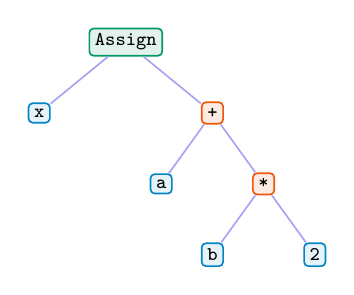
\begin{tikzpicture}[
  level distance=9mm,
  level 1/.style={sibling distance=22mm},
  level 2/.style={sibling distance=13mm},
  every node/.style={draw=ink, rounded corners=1.5pt, fill=card, font=\scriptsize\ttfamily, inner sep=2pt, line width=0.6pt},
  st/.style={draw=emerald, fill=emerald!12},
  ex/.style={draw=orangeC, fill=orangeC!12},
  lf/.style={draw=sky, fill=sky!10},
  edge from parent/.style={draw=indigo!50, line width=0.6pt}]
  \node[st] (as) {Assign}
    child {node[lf] (x) {x}}
    child {node[ex] (pl) {+}
      child {node[lf] (a) {a}}
      child {node[ex] (mu) {*}
        child {node[lf] (b) {b}}
        child {node[lf] (two) {2}}}};
\end{tikzpicture}
\begin{tikzpicture}[overlay, remember picture]\end{tikzpicture}
\vspace{1mm}

\footnotesize
\begin{tabular}{@{}ll@{}}
\toprule
Attribute & Flow on \tm{x = a + b * 2;} \\
\midrule
$\Gamma$ (inherited) & passed down to every leaf; resolves \tm{x}, \tm{a}, \tm{b} \\
$\tau$ (synthesised) & leaves \tm{int}; \tm{*}, \tm{+} give \tm{int}; Assign checks \\
$\mathit{in}$ (inherited) & builds \tm{a + (b*2)} left-associatively \\
unique name & \tm{x}, \tm{a}, \tm{b}; a second \tm{i} becomes \tm{i\#1} \\
\bottomrule
\end{tabular}
\caption{Attributed AST of a simple assignment, coloured as in the GUI:
statements green, expressions orange, leaves blue. The environment flows
down, types flow up, and each identifier is bound to a unique IR name.}
\label{fig:ast}
\end{figure}

\subsection{Three-address code and control flow}

The AST is lowered by a syntax-directed translation into three-address
code whose instructions have the forms $x=y\ \mathit{op}\ z$,
$x=\mathit{op}\ y$, $x=y$, $x=a[i]$, $a[i]=y$, \tm{goto} $L$,
\tm{if} $x$ \tm{goto} $L_t$ \tm{else} $L_f$, \tm{param}, \tm{call},
\tm{return}, \tm{print} and \tm{input}. Conditions are translated as
jumping code~\cite{aho2006dragon}: with true and false targets $t,f$,
\begin{equation}
\begin{aligned}
\mathcal{J}\llbracket B_1 \,\tm{\&\&}\, B_2\rrbracket(t,f) &=
 \mathcal{J}\llbracket B_1\rrbracket(L,f)\ ;\ L{:}\ \mathcal{J}\llbracket B_2\rrbracket(t,f),\\
\mathcal{J}\llbracket B_1 \,\tm{||}\, B_2\rrbracket(t,f) &=
 \mathcal{J}\llbracket B_1\rrbracket(t,L)\ ;\ L{:}\ \mathcal{J}\llbracket B_2\rrbracket(t,f),\\
\mathcal{J}\llbracket \tm{!}B\rrbracket(t,f) &= \mathcal{J}\llbracket B\rrbracket(f,t),
\end{aligned}
\label{eq:jump}
\end{equation}
with $L$ a fresh label, so short-circuit evaluation is exact and no
Boolean value is materialised unless it is stored. Basic blocks are
maximal sequences with a single entry and a single exit. The CFG is
cleaned of unreachable blocks and its critical edges are split, so that
copies inserted later on an edge have a block of their own. Dominators
are computed by the Cooper--Harvey--Kennedy iterative algorithm over
reverse postorder~\cite{cooper2001dom}, natural loops are identified
from back edges $n\to h$ with $h \operatorname{dom} n$, and each block
gets a loop depth. Fig.~\ref{fig:tac} shows the TAC and optimised SSA
the compiler produces for a small loop.

\begin{figure}[t]
\centering
\begin{minipage}[t]{0.47\columnwidth}
\scriptsize\textbf{TAC}\vspace{-1mm}
\begin{verbatim}
entry: n = input()
       s = 0
       i = 0
for1:  t2 = i < n
       if t2 goto body2
             else endfor4
body2: t3 = i % 3
       t4 = t3 == 0
       if t4 goto and7
             else endif6
and7:  t5 = i > 0
       if t5 goto then5
             else endif6
then5: s = s + i
endif6:
step3: i = i + 1
       goto for1
endfor4:
       print s
       return 0
\end{verbatim}
\end{minipage}\hfill
\begin{minipage}[t]{0.5\columnwidth}
\scriptsize\textbf{Optimised SSA}\vspace{-1mm}
\begin{verbatim}
entry: n = input()
       goto for1
for1:  i.2 = phi(0, i.3)
       s.2 = phi(0, s.4)
       if i.2 < n goto body2
             else endfor4
body2: t3 = i.2 % 3
       if t3 == 0 goto and7
             else endif6
and7:  if i.2 > 0 goto then5
             else endif6
then5: s.3 = s.2 + i.2
endif6:
       s.4 = phi(s.2, s.2, s.3)
       i.3 = i.2 + 1
       goto for1
endfor4:
       print s.2
       return 0
\end{verbatim}
\end{minipage}
\caption{Compiler output for
\tm{for(i=0;i<n;i++) if(i\%3==0 \&\& i>0) s+=i;}. Jumping code realises
\tm{\&\&}; after SSA and optimisation, comparisons are fused into
branches and constants into $\varphi$ arguments (split critical-edge
blocks omitted).}
\label{fig:tac}
\end{figure}

\subsection{SSA construction and optimisation}

Liveness is the least fixpoint of
\begin{equation}
\begin{aligned}
\mathit{LiveIn}(b)&=\mathit{use}(b)\cup\big(\mathit{LiveOut}(b)\setminus\mathit{def}(b)\big),\\
\mathit{LiveOut}(b)&=\textstyle\bigcup_{s\in\mathit{succ}(b)}\mathit{LiveIn}(s),
\end{aligned}
\label{eq:liveness}
\end{equation}
solved by a worklist over reverse postorder, with $\varphi$-uses
attributed to the corresponding predecessor edge. SSA is built by the
method of Cytron et~al.~\cite{cytron1991ssa}: for each variable $x$ with
definition blocks $D_x$, a $\varphi$ is placed at every block of the
iterated dominance frontier $\mathit{DF}^{+}(D_x)$ at which $x$ is live
on entry (pruned SSA), and variables are renamed by a walk of the
dominator tree. A read with no reaching definition becomes the
constant~0, which matches MiniC's zero-initialisation of locals.

The optimiser iterates, to a fixpoint or ten rounds, sparse conditional
constant propagation over the lattice
$\top \sqsupset c \sqsupset \bot$ with executable-edge tracking
(SCCP)~\cite{wegman1991sccp}, copy propagation, algebraic simplification
and strength reduction (for example $x\cdot 2^m\Rightarrow x\ll m$,
$x+0\Rightarrow x$), global value numbering scoped by the dominator
tree, dead-code elimination over SSA def-use chains and the merging of
straight-line blocks. It then splits critical edges again and fuses
each comparison with the branch that consumes it into a compare-branch
instruction. Semantic preservation is checked on every benchmark by
executing the SSA program before and after optimisation and comparing
outputs.

\subsection{Profiling and transition probabilities}

The optimised SSA program is executed by a reference interpreter with
bounds-checked memory on a training input. The interpreter counts every
CFG edge $n(b,s)$, and the profiled transition matrix is
\begin{equation}
P_{\mathrm{prof}}(b,s)=\frac{n(b,s)}{\sum_{s'\in\mathit{succ}(b)} n(b,s')},
\label{eq:pprof}
\end{equation}
falling back to the static prior for blocks never reached in training.
The Static-Prior variant uses the classical loop heuristic~\cite{wu1994}
instead: if exactly one successor leaves a loop containing $b$,
\begin{equation}
P_{\mathrm{stat}}(b,s)=\begin{cases}
0.1 & s \text{ exits the loop},\\
0.9 & \text{otherwise},
\end{cases}
\label{eq:pstat}
\end{equation}
and otherwise $P_{\mathrm{stat}}(b,s)=1/|\mathit{succ}(b)|$.
Fig.~\ref{fig:cfg} contrasts the two on the inner loop of the
rare-branch benchmark, where an error path is taken in about 1\% of
iterations but the static prior sees a fair coin.

\begin{figure}[t]
\centering
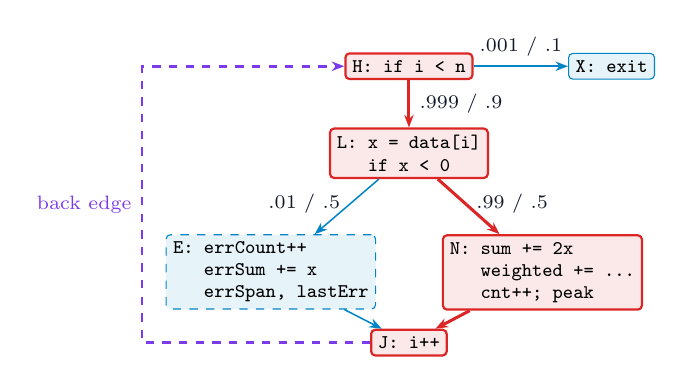
\begin{tikzpicture}[node distance=6mm and 7mm, font=\scriptsize]
  \node[blk, draw=redC, fill=redC!10, line width=0.8pt] (h) {H: if i < n};
  \node[blk, below=of h, draw=redC, fill=redC!10, line width=0.8pt] (l) {L: x = data[i]\\\ \ \ if x < 0};
  \node[blk, below left=7mm and -6mm of l, draw=sky, fill=sky!10, dashed] (e) {E: errCount++\\\ \ \ errSum += x\\\ \ \ errSpan, lastErr};
  \node[blk, below right=7mm and -6mm of l, draw=redC, fill=redC!10, line width=0.8pt] (n) {N: sum += 2x\\\ \ \ weighted += ...\\\ \ \ cnt++; peak};
  \node[blk, below=19mm of l, draw=redC, fill=redC!10, line width=0.8pt] (j) {J: i++};
  \node[blk, right=12mm of h, draw=sky, fill=sky!10] (x) {X: exit};
  \draw[flow, draw=redC, line width=1.1pt] (h) -- node[right,align=left,text=ink]{.999 / .9} (l);
  \draw[flow, draw=sky] (h) -- node[above,text=ink]{.001 / .1} (x);
  \draw[flow, draw=sky] (l) -- node[left, pos=0.45,text=ink]{.01 / .5} (e);
  \draw[flow, draw=redC, line width=1.1pt] (l) -- node[right, pos=0.45,text=ink]{.99 / .5} (n);
  \draw[flow, draw=sky] (e) -- (j);
  \draw[flow, draw=redC, line width=1.1pt] (n) -- (j);
  \draw[flow, draw=violet, dashed, line width=1pt] (j.west) -- ($(j.west -| e.west)+(-3mm,0)$) |- node[pos=0.25,left,text=violet]{back edge} (h.west);
\end{tikzpicture}
\caption{Inner loop of the rare-branch benchmark. Edge labels give
$P_{\mathrm{prof}}/P_{\mathrm{stat}}$. Red marks the hot path found by
profiling and blue the rarely executed blocks: the error block E runs in
1\% of iterations, whereas the static prior assumes 50\%.}
\label{fig:cfg}
\end{figure}

\subsection{The residency MDP of a value}

\begin{definition}[Residency MDP]
For an SSA value $v$ with live range $L_v\subseteq B$, the residency MDP
has states $(b,s)$ with $b\in L_v$ and $s\in\{\Reg,\Mem\}$ (control is in
block $b$ and $v$ is in a register or in its slot). In state $\Reg$ the
actions are \emph{stay} and \emph{spill} (cost $\cst$); in state $\Mem$
they are \emph{stay} and \emph{reload} (cost $\cld$). Control moves from
$b$ to $b'\in L_v$ with probability $P(b,b')$ when $v\in\mathit{LiveIn}(b')$;
leaving the live range is absorbing with value $0$.
\end{definition}

Let $u_v(b)$, $d_v(b)$ and $f_v(b)$ be the numbers of uses,
definitions and \emph{forwardable} uses (a use immediately after the
definition, which the peephole pass turns into a register move when $v$
is spilled) of $v$ in $b$, and $c_v(b)$ the number of calls in $b$
across which $v$ is live. The per-block rewards are
\begin{equation}
\begin{aligned}
r_\Reg(b) &= \csv\,\big(u_v(b)+d_v(b)+f_v(b)\big)-c_v(b)\,(\cst+\cld),\\
r_\Mem(b) &= -\big(u_v(b)\,\cld + d_v(b)\,\cst + f_v(b)\,\cmv\big),
\end{aligned}
\label{eq:reward}
\end{equation}
with $\csv$ a small bonus for a register access, $\cmv$ the cost of a
forwarded move and an extra $-\cld$ in the definition block of a
parameter, which arrives in its slot. The optimal values satisfy the
Bellman equations~\cite{bellman1957,puterman1994}
\begin{equation}
\begin{aligned}
V(b,\Reg) &= r_\Reg(b) + \max\big\{\bar V_\Reg(b),\ -\cst + \bar V_\Mem(b)\big\},\\
V(b,\Mem) &= r_\Mem(b) + \max\big\{\bar V_\Mem(b),\ -\cld + \bar V_\Reg(b)\big\},\\
\bar V_s(b) &= \textstyle\sum_{b'\in L_v} P(b,b')\,V(b',s),
\end{aligned}
\label{eq:bellman}
\end{equation}
Fig.~\ref{fig:mdp} draws the two states. Because a live range is left
with probability one under every policy of a terminating program, the
chain restricted to $L_v$ is transient and (\ref{eq:bellman}) is solved
undiscounted, as a total-reward MDP. For a fixed policy $\pi$, policy
evaluation is the sparse linear system
\begin{equation}
\big(I-P_\pi\big)\,V_\pi = r_\pi ,
\label{eq:policyeval}
\end{equation}
where $P_\pi$ is substochastic and transient, so $I-P_\pi$ is a
non-singular M-matrix and Gaussian elimination without pivoting is
stable. Howard's policy iteration~\cite{howard1960} alternates
(\ref{eq:policyeval}) with greedy improvement and terminates in a finite
number of rounds with the exact optimum; we keep value iteration as an
independent cross-check in the test suite. If the restricted chain
were ever not transient, the solver would fall back to a discount factor
$\gamma=0.999$.

\begin{figure}[t]
\centering
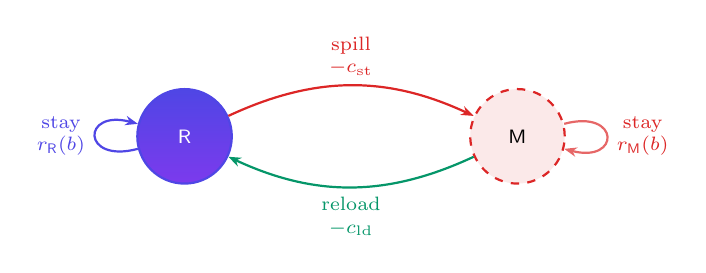
\begin{tikzpicture}[font=\scriptsize, >=Stealth]
  \node[circle, draw=indigo, top color=indigo, bottom color=violet, text=white, minimum size=12mm, line width=0.8pt] (r) {$\Reg$};
  \node[circle, draw=redC, fill=redC!10, minimum size=12mm, line width=0.8pt, dashed, right=30mm of r] (m) {$\Mem$};
  \draw[flow, draw=redC, line width=0.8pt] (r) to[bend left=25] node[above,align=center,text=redC]{spill\\$-\cst$} (m);
  \draw[flow, draw=emerald, line width=0.8pt] (m) to[bend left=25] node[below,align=center,text=emerald]{reload\\$-\cld$} (r);
  \draw[flow, draw=indigo, line width=0.8pt] (r) to[loop left, looseness=6] node[left,align=center,text=indigo]{stay\\$r_\Reg(b)$} (r);
  \draw[flow, draw=redC!70, line width=0.8pt] (m) to[loop right, looseness=6] node[right,align=center,text=redC]{stay\\$r_\Mem(b)$} (m);
\end{tikzpicture}
\caption{The two-state residency MDP replicated over each block $b$ of a
value's live range. In either state control moves to $b'$ with
probability $P(b,b')$; leaving $L_v$ is absorbing with value 0.
Rewards follow (\ref{eq:reward}).}
\label{fig:mdp}
\end{figure}

\subsection{Expected gain of a value}

An auction loser does not choose its policy: it is forced to stay in
$\Mem$ throughout. Let $V_{\mathrm{mem}}$ be the value of that forced
policy, obtained from (\ref{eq:policyeval}) with $\pi\equiv$ \emph{stay}.
The per-entry gain is the difference between entering the live range
with a register under the optimal policy and entering it without one,
$g(v)=V^\ast(\mathit{def}(v),\Reg)-V_{\mathrm{mem}}(\mathit{def}(v),\Mem)$.
The live range is entered once for each execution of the definition
block, whose expected count per invocation $\phi$ solves the
Markov-chain flow equations
\begin{equation}
\phi = e_{b_0} + P^{\top}\phi ,
\label{eq:freq}
\end{equation}
so the expected register-residency gain of $v$ per invocation is
\begin{equation}
G(v)=\phi\big(\mathit{def}(v)\big)\cdot
\Big(V^\ast\big(\mathit{def}(v),\Reg\big)-V_{\mathrm{mem}}\big(\mathit{def}(v),\Mem\big)\Big).
\label{eq:gain}
\end{equation}
Measuring against $V_{\mathrm{mem}}$ rather than against
$V^\ast(\cdot,\Mem)$ matters: an optimal policy that starts in $\Mem$
may reload at once, which would cap every gain at roughly $\cld$ and
hide the difference between hot and cold values.
$G(v)$ is the quantity a compiler engineer would ask for (expected
cycles saved), and the GUI shows it for every value. In the rare-branch
example of Fig.~\ref{fig:cfg}, the profiled MDP rates the hot-path
accumulators \tm{cnt.3} and \tm{weighted.3} at $G=20{,}300$ and the
error-path counters \tm{errSum.3} and \tm{errCount.3} at $G=180$, a
factor of 113. Under the static prior (\ref{eq:pstat}) all four receive
the same gain, 202.5, because the two arms of the branch look alike;
Static-Prior consequently keeps the error-path value \tm{lastErr} in a
register and spills \tm{cnt} and \tm{weighted}, whereas \MG\ does the
opposite.

\subsection{Coalitions on $\varphi$-webs}

A loop-carried variable is a chain of SSA values joined by
$\varphi$-functions. If they are allocated independently, the auction
may grant a register to one version and not the next, and every
traversal of the back edge then pays a copy through memory. We
therefore form coalitions by union-find over $\varphi$ edges, merging
the argument $a$ and result $p$ of a $\varphi$ in block $h$ along edge
$(b,h)$ only when the edge is \emph{hot}:
\begin{equation}
\phi(b)\,P(b,h) \;\ge\; \theta\cdot\max\big\{\phi(\mathit{def}(a)),\ \phi(h)\big\},
\qquad \theta=0.25 .
\label{eq:hot}
\end{equation}
A loop-carried variable thus forms one coalition around its back edge,
while a copy made once on loop entry, or on a rare path, does not drag
a cold value into a hot coalition. Every member of coalition $C$ bids the
coalition's total gain,
\begin{equation}
\beta(v)=\sum_{w\in C(v)} G(w),
\label{eq:bid}
\end{equation}
so the coalition wins or loses as a unit. This is the transferable-utility
view of cooperative game theory~\cite{shapley1953}: the coalition's
value is what its members achieve together, and (\ref{eq:bid}) lets
members with small individual gains (for example the version of
\tm{i} after the increment, $G=12{,}288$) inherit the bid of the whole
web ($\beta=94{,}223$).

\subsection{Sealed-bid auction on the chordal interference graph}

The interference graph $\mathcal{I}=(V,A)$ joins two values when one is
live at the definition of the other. On strict SSA $\mathcal{I}$ is
chordal~\cite{hack2006ssa}; we compute a maximum cardinality search
order $\sigma$~\cite{tarjan1984} and verify on every function that its
reverse is a perfect elimination ordering (PEO), which held for all
functions in our suite. In a chordal graph visited in MCS order, the
already-visited neighbours of each vertex form a clique, so when $v$
arrives its already-visited neighbours together with $v$ are a clique
$Q_v$, a set of values that are all simultaneously live.

The auction (Algorithm~\ref{alg:auction}) visits values in order
$\sigma$. If $v$ has fewer than $k$ already-winning neighbours, it wins
outright. Otherwise $Q_v$ exceeds the register budget and a sealed-bid
round awards the $k$ registers of that clique to the $k$ highest bids:
\begin{equation}
W(Q_v) = \arg\max_{S\subseteq Q_v,\ |S|\le k}\ \sum_{w\in S}\beta(w),
\label{eq:auction}
\end{equation}
which for a single capacity constraint is solved exactly by sorting.
Ties are broken by $\sigma$, so the result is deterministic. Losers are
spilled to slots that are shared by every member of a $\varphi$-web,
so that spilled $\varphi$ copies become no-ops. Registers are then bound
along $\sigma$, choosing for each winner a register not held by any
winning neighbour and preferring one already held by a member of its
web, so the $\varphi$ copy disappears. Fig.~\ref{fig:auction} shows a
real auction round from the rare-branch benchmark at $k=4$.

\begin{figure}[t]
\centering
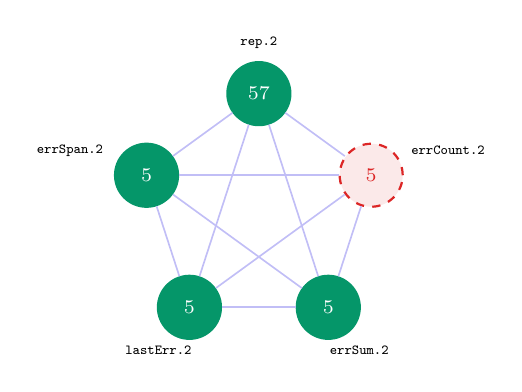
\begin{tikzpicture}[font=\scriptsize]
  \foreach \name/\lab/\bid/\ang/\win in {
      a/rep.2/57/90/1, b/errSpan.2/5/162/1, c/lastErr.2/5/234/1,
      d/errSum.2/5/306/1, e/errCount.2/5/18/0} {
    \ifnum\win=1
      \node[circle, draw=emerald, fill=emerald, text=white, minimum size=8mm, inner sep=0pt, line width=0.8pt]
        (\name) at (\ang:15mm) {\bid};
    \else
      \node[circle, draw=redC, dashed, fill=redC!10, text=redC, minimum size=8mm, inner sep=0pt, line width=0.8pt]
        (\name) at (\ang:15mm) {\bid};
    \fi
    \node[font=\tiny\ttfamily, anchor=\ang+180] at (\ang:19.5mm) {\lab};
  }
  \foreach \u/\v in {a/b,a/c,a/d,a/e,b/c,b/d,b/e,c/d,c/e,d/e}
    \draw[draw=indigo!35, line width=0.6pt] (\u) -- (\v);
\end{tikzpicture}
\caption{An auction round at $k=4$ in the rare-branch benchmark:
when \tm{errCount.2} arrives in MCS order its clique has five members.
Node labels are bids $\beta$; the four highest win (green), and the tie
at 5 is broken by MCS order, so \tm{errCount.2} is spilled (red, dashed).
The GUI uses the same colours for auction winners and losers.}
\label{fig:auction}
\end{figure}

\begin{algorithm}[t]
\caption{Profile-driven gains and coalition bids}
\label{alg:gains}
\begin{algorithmic}[1]
\REQUIRE SSA function with CFG $\mathcal{C}$, edge counts $n$ (or none)
\ENSURE gains $G$, bids $\beta$, coalitions $C$
\STATE $P \leftarrow$ (\ref{eq:pprof}) if $n$ given, else (\ref{eq:pstat})
\STATE $\phi \leftarrow$ solve $(I-P^\top)\phi=e_{b_0}$ \hfill (\ref{eq:freq})
\FORALL{$v\in V$}
  \STATE build rewards $r_\Reg, r_\Mem$ on $L_v$ \hfill (\ref{eq:reward})
  \STATE $\pi \leftarrow$ \emph{stay} in every state
  \REPEAT
    \STATE $V_\pi \leftarrow$ solve $(I-P_\pi)V_\pi=r_\pi$ \hfill (\ref{eq:policyeval})
    \STATE $\pi' \leftarrow$ greedy in (\ref{eq:bellman}) w.r.t.\ $V_\pi$
    \STATE \textbf{if} $\pi'=\pi$ \textbf{then break}; $\pi\leftarrow\pi'$
  \UNTIL{false}
  \STATE $V_{\mathrm{mem}} \leftarrow$ evaluate $\pi\equiv$\,\emph{stay} from $\Mem$
  \STATE $g\leftarrow V_\pi(\mathit{def}(v),\Reg)-V_{\mathrm{mem}}(\mathit{def}(v),\Mem)$
  \STATE $G(v)\leftarrow \phi(\mathit{def}(v))\cdot g$ \hfill (\ref{eq:gain})
\ENDFOR
\STATE $C \leftarrow$ union-find over $\varphi$ edges satisfying (\ref{eq:hot})
\STATE $\beta(v)\leftarrow\sum_{w\in C(v)}G(w)$ for all $v$ \hfill (\ref{eq:bid})
\RETURN $G,\beta,C$
\end{algorithmic}
\end{algorithm}

\begin{algorithm}[t]
\caption{MCS-ordered sealed-bid auction and register binding}
\label{alg:auction}
\begin{algorithmic}[1]
\REQUIRE interference graph $\mathcal{I}$, bids $\beta$, $k$, webs
\ENSURE allocation $\rho$
\STATE $\sigma\leftarrow$ \textsc{MaximumCardinalitySearch}$(\mathcal{I})$; assert reverse$(\sigma)$ is a PEO
\STATE $\mathit{win}\leftarrow\emptyset$
\FORALL{$v$ in order $\sigma$}
  \STATE $R\leftarrow\{w\in\mathrm{adj}(v)\mid w\in\mathit{win}\}$
  \IF{$|R|<k$}
    \STATE $\mathit{win}\leftarrow\mathit{win}\cup\{v\}$
  \ELSE
    \STATE $Q\leftarrow R\cup\{v\}$ \COMMENT{a clique}
    \STATE $S\leftarrow$ top-$k$ of $Q$ by $(\beta,-\sigma)$ \hfill (\ref{eq:auction})
    \STATE $\mathit{win}\leftarrow(\mathit{win}\setminus Q)\cup S$
  \ENDIF
\ENDFOR
\FORALL{$v\in\mathit{win}$ in order $\sigma$}
  \STATE $F\leftarrow\{0..k{-}1\}\setminus\{\rho(w)\mid w\in\mathrm{adj}(v)\}$
  \STATE $\rho(v)\leftarrow$ a register of $F$ held by $v$'s web, else $\min F$
\ENDFOR
\RETURN $\rho$ (values without a register are spilled)
\end{algorithmic}
\end{algorithm}

\subsection{Best-response dynamics and equilibrium}

The auction decides each clique locally, so a loser can end up with a
register that none of its neighbours actually uses (for example
because a rival that beat it later lost elsewhere). We model the result
as a game whose players are coalitions, whose strategies are a
register for each member or memory, and whose payoff is $\beta$ when
all members hold registers and $0$ otherwise, subject to the
non-interference constraint. A spilled coalition $C$ has a profitable
unilateral deviation if
\begin{equation}
\beta(C)>0\ \wedge\ \forall v\in C:\ \{0,\dots,k{-}1\}\setminus\rho\big(\mathrm{adj}(v)\big)\neq\emptyset .
\label{eq:nash}
\end{equation}
Best-response dynamics (Algorithm~\ref{alg:br}) let deviating
coalitions take free registers, highest bid first, until none can.

Splitting a coalition between registers and memory costs a copy through
memory on each hot $\varphi$ edge that joins a winner and a loser. When
that expected penalty is at least the winners' own gain,
\begin{equation}
\sum_{\substack{(b,h)\ \varphi\text{-edge}\\ \text{split}}}\phi(b)\,P(b,h)\,c_{(b,h)}
\;\ge\;\sum_{w\in C,\ \rho(w)\neq\bot}G(w),
\label{eq:repair}
\end{equation}
with $c_{(b,h)}$ equal to $\cld$ or $\cst$ depending on the direction of
the copy, the winners concede and the whole coalition leaves the
game, after which best response runs again to reuse the freed
registers.

\begin{proposition}
Algorithm~\ref{alg:br} terminates after at most $|V|$ deviations, and
its result is a pure Nash equilibrium of the coalition game: no spilled
coalition satisfies (\ref{eq:nash}), and no winning coalition can raise
its payoff by deviating.
\end{proposition}
\begin{proofsketch}
A deviation moves a whole coalition from memory into registers that
are free with respect to all of its neighbours, without evicting
anyone, so the set of allocated values grows strictly; hence at most
$|V|$ deviations occur. Repair only removes values, and the final
best-response pass again ends when (\ref{eq:nash}) fails for every
spilled coalition. A winning coalition already receives its maximal
payoff $\beta(C)$, and changing to another free register leaves the
payoff unchanged, so no player has a strictly profitable deviation.
\end{proofsketch}

The equilibrium need not maximise (\ref{eq:objective}) globally, since
the register game is a congestion game~\cite{rosenthal1973} with many
equilibria. The auction is what steers the dynamics towards the
high-gain equilibrium: best response only fills registers that the
auction left free.

\begin{algorithm}[t]
\caption{Best-response dynamics with coalition repair}
\label{alg:br}
\begin{algorithmic}[1]
\REQUIRE $\rho$ from Algorithm~\ref{alg:auction}, coalitions $C$, bids $\beta$, gains $G$
\ENSURE equilibrium allocation $\rho$
\STATE \textsc{BestResponse}$(\rho)$
\FORALL{coalitions $C$ split between registers and memory}
  \IF{(\ref{eq:repair}) holds for $C$}
    \STATE $\rho(w)\leftarrow\bot$ for every $w\in C$
  \ENDIF
\ENDFOR
\STATE \textbf{if} anything was demoted \textbf{then} \textsc{BestResponse}$(\rho)$
\RETURN $\rho$
\item[]
\item[] \textbf{procedure} \textsc{BestResponse}$(\rho)$
\REPEAT
  \STATE $\mathit{changed}\leftarrow$ false
  \FORALL{spilled coalitions $C$ by decreasing $\beta$}
    \IF{every $v\in C$ has a free register (\ref{eq:nash})}
      \STATE assign them, preferring registers of web partners
      \STATE $\mathit{changed}\leftarrow$ true
    \ENDIF
  \ENDFOR
\UNTIL{not $\mathit{changed}$}
\end{algorithmic}
\end{algorithm}

\begin{figure*}[!t]
\centering
\IfFileExists{gui_allocation.png}{%
  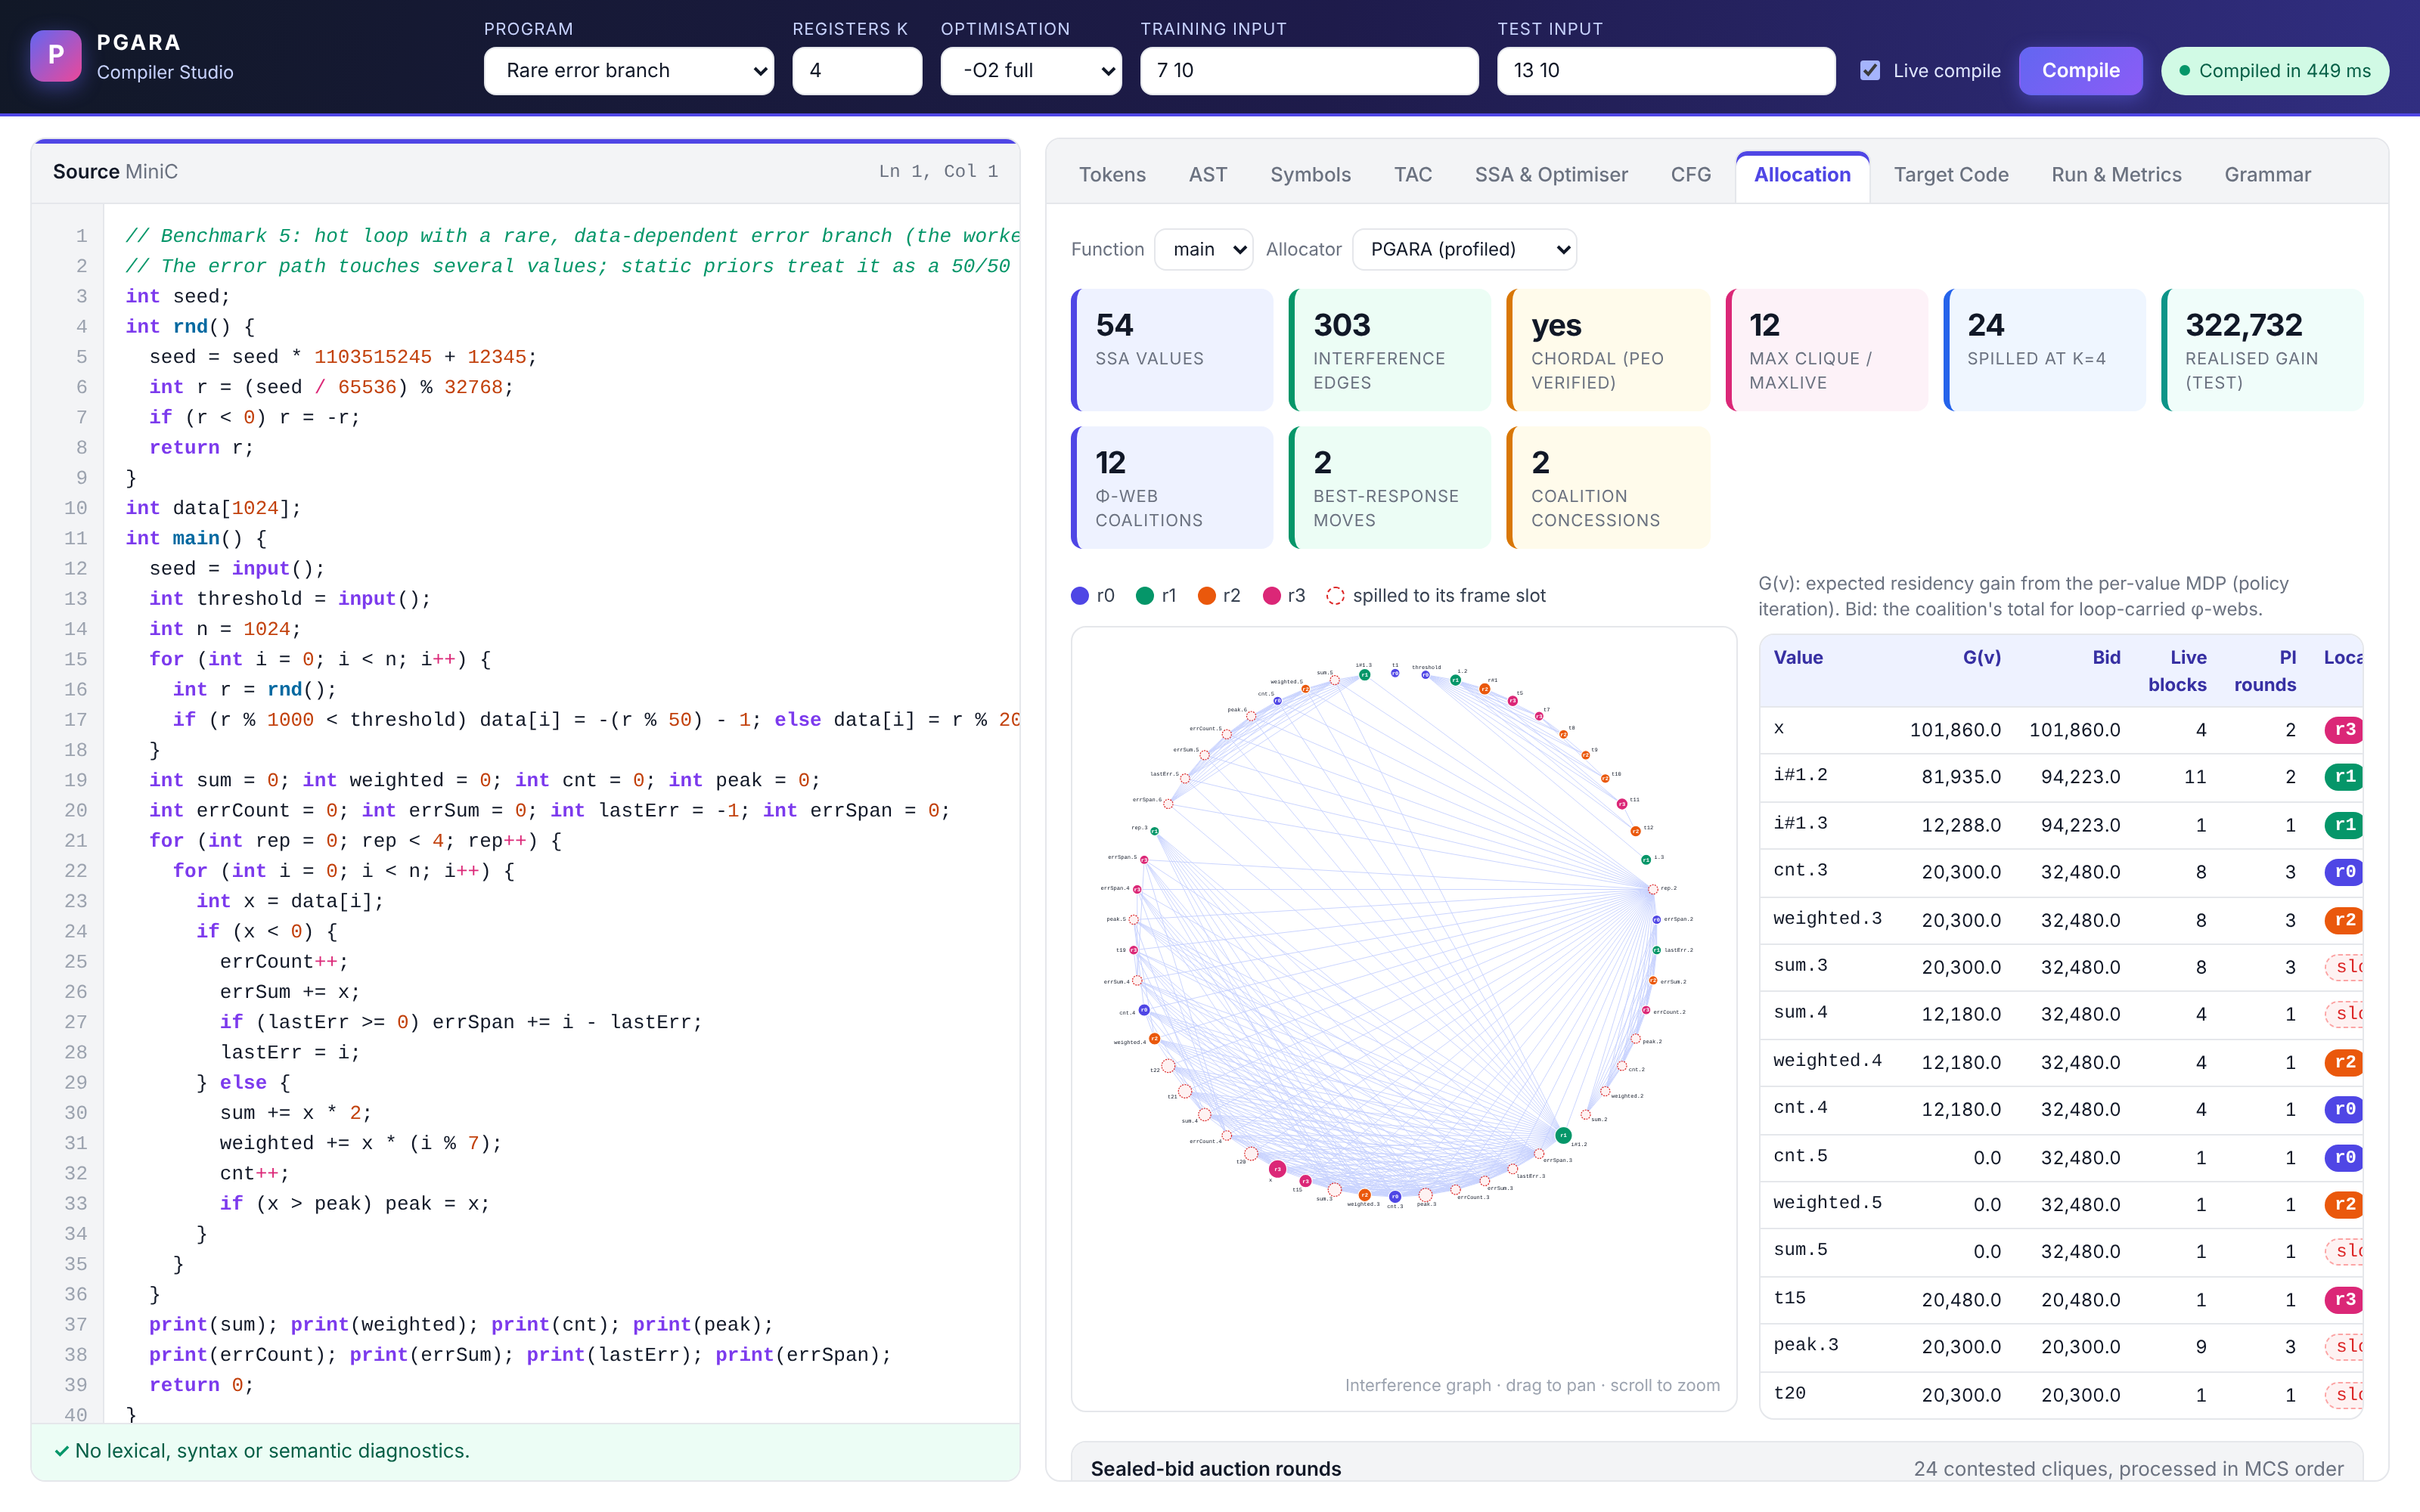
\includegraphics[width=0.92\textwidth]{gui_allocation.png}%
}{%
  \fbox{\parbox[c][60mm][c]{0.9\textwidth}{\centering\small
  Screenshot of the Allocation view (gui\_allocation.png).}}%
}
\caption{The \MG\ Compiler Studio on the rare-branch benchmark at
$k=4$. Left: the MiniC editor with syntax colouring and diagnostics.
Right: the Allocation view with the interference graph (one colour per
register, red dashed outline for spilled values), each value's gain
$G(v)$, coalition bid, live-range size, policy-iteration rounds and
register, and the auction rounds in MCS order with winners in green and
losers in red.}
\label{fig:gui}
\end{figure*}

\subsection{Back end: leaving SSA and code generation}

Fig.~\ref{fig:allocflow} summarises the allocation flow and its
hand-off to the back end. The target, PG-RISC, is a load/store RISC with
allocatable registers $r_0,\dots,r_{k-1}$, three scratch registers
$t_0$--$t_2$ for spilled operands, a return-value register and a frame
pointer. The frame holds parameters, spill slots (one per $\varphi$-web),
caller-save slots and local arrays. $\varphi$-functions are replaced by
parallel copies on the (already split) incoming edges, sequentialised
with cycles broken through $t_2$; copies between values that share a
register or a slot vanish. Registers live across a call are saved and
restored around it. A peephole pass threads jumps, removes jumps to the
next instruction and forwards a store to an immediately following load
of the same slot, turning the load into a move or deleting it, which
is the forwarding that $f_v(b)$ in (\ref{eq:reward}) anticipates.

\begin{figure}[t]
\centering
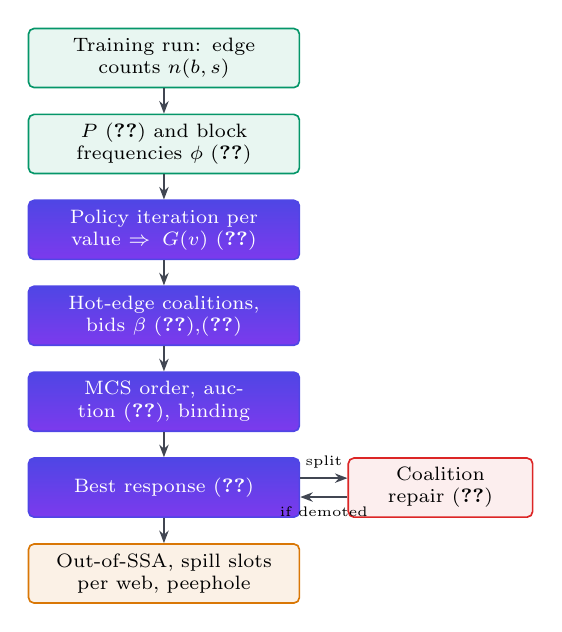
\begin{tikzpicture}[node distance=3.2mm, font=\scriptsize]
  \node[midst, text width=33mm] (a) {Training run: edge counts $n(b,s)$};
  \node[midst, text width=33mm, below=of a] (b) {$P$ (\ref{eq:pprof}) and block frequencies $\phi$ (\ref{eq:freq})};
  \node[hot, text width=33mm, below=of b] (c) {Policy iteration per value $\Rightarrow G(v)$ (\ref{eq:gain})};
  \node[hot, text width=33mm, below=of c] (d) {Hot-edge coalitions, bids $\beta$ (\ref{eq:hot}),(\ref{eq:bid})};
  \node[hot, text width=33mm, below=of d] (e) {MCS order, auction (\ref{eq:auction}), binding};
  \node[hot, text width=33mm, below=of e] (f) {Best response (\ref{eq:nash})};
  \node[back, text width=33mm, below=of f] (g) {Out-of-SSA, spill slots per web, peephole};
  \node[stage, draw=redC, fill=redC!8, text width=22mm, right=6mm of f] (r) {Coalition repair (\ref{eq:repair})};
  \foreach \x/\y in {a/b,b/c,c/d,d/e,e/f,f/g} \draw[flow] (\x) -- (\y);
  \draw[flow] ($(f.east)+(0,1.2mm)$) -- node[above,font=\tiny]{split} ($(r.west)+(0,1.2mm)$);
  \draw[flow] ($(r.west)+(0,-1.2mm)$) -- node[below,font=\tiny]{if demoted} ($(f.east)+(0,-1.2mm)$);
\end{tikzpicture}
\caption{Flow of the \MG\ allocator, from profile to target code.}
\label{fig:allocflow}
\end{figure}

\subsection{Modules and the team's contribution}

The work divides into five modules, each owned by one team member (the
full list is given in the contributions section). The core pipeline
module provides the lexer, the grammar and its LL(1) verification, the
parser and AST, and TAC generation (Shreyans Chowdry). The semantic
module provides the scoped symbol table, the attribute evaluation and
diagnostics (Samrender Singh Saini). The optimisation and code-generation
module provides SSA, the optimiser, the \MG\ allocator and PG-RISC code
generation (Karthikeya Jami). The runtime and evaluation module provides
the interpreter, the simulator, the test suite and the benchmark
harness (Abhishek Kumar). The interface module provides the web GUI,
the visualisations and the documentation (Nishanth Kumar).

\newcommand{\guishot}[2]{%
  \IfFileExists{#1}{\includegraphics[width=\linewidth]{#1}}{%
  \fbox{\parbox[c][40mm][c]{0.95\linewidth}{\centering\small #2}}}}
\begin{figure*}[!t]
\centering
\begin{minipage}[t]{0.49\textwidth}\centering
\guishot{gui_pane_tokens.png}{Tokens view}\\[-1pt]
{\footnotesize (a) Tokens: the DFA's token stream, coloured by kind}
\end{minipage}\hfill
\begin{minipage}[t]{0.49\textwidth}\centering
\guishot{gui_small_ast.png}{AST view}\\[-1pt]
{\footnotesize (b) AST: declarations, control flow, statements, expressions and leaves}
\end{minipage}\\[5pt]
\begin{minipage}[t]{0.49\textwidth}\centering
\guishot{gui_small_cfg.png}{CFG view}\\[-1pt]
{\footnotesize (c) CFG: block headers coloured by execution frequency, edges labelled
$P_{\mathrm{prof}}$ ($P_{\mathrm{stat}}$)}
\end{minipage}\hfill
\begin{minipage}[t]{0.49\textwidth}\centering
\guishot{gui_pane_run.png}{Run \& Metrics view}\\[-1pt]
{\footnotesize (d) Run \& Metrics: reference output and the four allocators compared}
\end{minipage}
\caption{Further views of the \MG\ Compiler Studio. (a) and (d) show
the rare-branch benchmark; (b) and (c) show the loop of
Fig.~\ref{fig:tac} compiled with training input 10.}
\label{fig:guitabs}
\end{figure*}

%% =====================================================================
\section{Implementation and Result Analysis}
\label{sec:impl}

\subsection{Tools and setup}

The compiler is written in Python~3 using only the standard library, so
it runs on any machine with a recent Python installation and no package
manager~\cite{python}. A small HTTP server from the standard library
serves the web interface and a JSON compilation endpoint; the interface
is plain HTML, CSS and JavaScript with hand-drawn SVG for trees and
graphs, using a colour code that is consistent across views (token
kinds, AST node categories, one colour per register, red for spills,
green for auction winners, and a blue-to-red heat scale for block
frequencies), so that the same colours used in the figures of this
paper appear on screen. The GUI
is started with a single start-up script, which launches the server on
port 8765 and opens the browser, and the benchmark study is run with one
command-line invocation that writes JSON and CSV results. A
\texttt{unittest} suite of 23 tests covers the lexer, grammar, parser,
semantic checks, SSA invariants (single assignment and dominance of
uses), optimiser semantic preservation, chordality, agreement of policy
and value iteration, a hand-computed gain, auction capacity, the Nash
property and end-to-end runs of all allocators for $k\in\{2,3,4,6\}$;
all tests pass. The interface was exercised end to end in headless
Chromium through Playwright~\cite{playwright}, which also produced the
screenshots in Figs.~\ref{fig:gui} and~\ref{fig:guitabs}.

Each benchmark is compiled at the full optimisation level, profiled on
a training input and measured on a different test input, for every
allocator and $k\in\{3,4,5,6,8\}$: 200 configurations. Every simulated
run is compared with the reference interpreter's output and all 200
match. Experiments ran on a Linux container with Python~3.13; because
the simulator counts cycles deterministically, the results do not
depend on the host.





\subsection{Parameters and benchmarks}

Table~\ref{tab:params} lists the parameters. The cost model matches the
simulator's latencies, so the gains are expressed in the same cycles
that are measured. The suite (Table~\ref{tab:bench}) spans straight-line
code, regular loops, recursion and programs whose control flow depends
on the data: a rare error branch, an early-exit search, a switch-like
dispatch chain and a token scanner. Most programs generate their data
with a linear congruential generator seeded from the input, so training
and test inputs exercise the same code with different data.

\begin{table}[t]
\centering
\caption{Parameter setup}
\label{tab:params}
\footnotesize
\begin{tabular}{@{}lr@{}}
\toprule
Parameter & Value \\
\midrule
Register budgets $k$ & 3, 4, 5, 6, 8 \\
Load / store cost $\cld$ / $\cst$ (cycles) & 4 / 2 \\
Register-access bonus $\csv$, forwarded move $\cmv$ & 1 / 1 \\
ALU / MUL / DIV latency & 1 / 3 / 12 \\
Taken / not-taken branch, call / return & 2 / 1, 3 / 3 \\
Discount $\gamma$ & 1 (fallback 0.999) \\
Static loop-stay probability & 0.9 \\
Hot-edge threshold $\theta$ & 0.25 \\
Optimiser rounds (max) & 10 \\
Interpreter / simulator step limits & $3\cdot10^6$ / $1.2\cdot10^7$ \\
Training $\neq$ test input & all benchmarks \\
\bottomrule
\end{tabular}
\end{table}

\begin{table}[t]
\centering
\caption{Benchmarks: SSA values, $\varphi$s, largest interference
clique $\omega$, mean and maximum policy-iteration rounds, and time
to run all four allocators ($k=4$)}
\label{tab:bench}
\footnotesize
\setlength{\tabcolsep}{3.5pt}
\begin{tabular}{@{}lrrrrrr@{}}
\toprule
Benchmark & $|V|$ & $\varphi$ & $\omega$ & PI$_{\text{mean}}$ & PI$_{\max}$ & ms \\
\midrule
straightline & 39 & 0 & 11 & 1.00 & 1 & 2.6 \\
arraysum & 38 & 16 & 9 & 1.29 & 3 & 6.2 \\
matmul & 51 & 10 & 8 & 1.27 & 3 & 5.9 \\
recursion & 39 & 4 & 7 & 1.28 & 3 & 4.4 \\
rarebranch & 62 & 30 & 12 & 1.26 & 3 & 9.4 \\
earlyexit & 41 & 17 & 10 & 1.29 & 3 & 8.0 \\
dispatch & 116 & 55 & 15 & 1.17 & 7 & 21.7 \\
scanner & 89 & 49 & 11 & 1.15 & 4 & 19.8 \\
sort & 53 & 16 & 10 & 1.32 & 3 & 11.9 \\
collatz & 30 & 16 & 9 & 1.53 & 3 & 9.6 \\
\bottomrule
\end{tabular}
\end{table}

\begin{figure*}[!t]
\centering
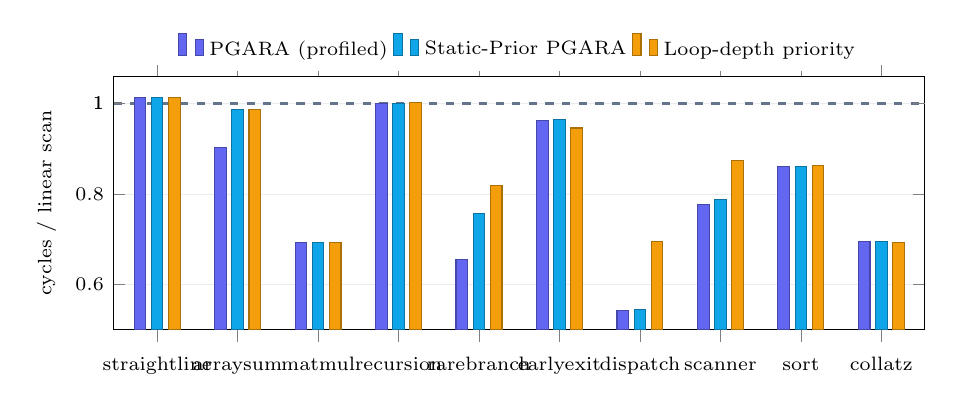
\begin{tikzpicture}
\begin{axis}[
  ybar, bar width=4.2pt, width=0.98\textwidth, height=48mm,
  ymin=0.5, ymax=1.06, ylabel={cycles / linear scan},
  symbolic x coords={straightline,arraysum,matmul,recursion,rarebranch,earlyexit,dispatch,scanner,sort,collatz},
  xtick=data, x tick label style={font=\scriptsize, text height=1.6ex, text depth=0.3ex},
  y tick label style={font=\scriptsize}, ylabel style={font=\scriptsize},
  legend style={font=\scriptsize, at={(0.5,1.02)}, anchor=south, legend columns=3, draw=none},
  ymajorgrids, grid style={draw=rule!80}, enlarge x limits=0.06,
  extra y ticks={1}, extra y tick style={grid=major, grid style={draw=cLS, dashed, line width=0.8pt}},
]
\addplot[fill=cPG, draw=cPG!70!black] coordinates {(straightline,1.014) (arraysum,0.903) (matmul,0.692) (recursion,1.001) (rarebranch,0.655) (earlyexit,0.962) (dispatch,0.542) (scanner,0.777) (sort,0.860) (collatz,0.695)};
\addplot[fill=cSP, draw=cSP!70!black] coordinates {(straightline,1.014) (arraysum,0.986) (matmul,0.692) (recursion,1.000) (rarebranch,0.757) (earlyexit,0.965) (dispatch,0.544) (scanner,0.787) (sort,0.860) (collatz,0.695)};
\addplot[fill=cLD, draw=cLD!70!black] coordinates {(straightline,1.014) (arraysum,0.986) (matmul,0.692) (recursion,1.002) (rarebranch,0.819) (earlyexit,0.946) (dispatch,0.696) (scanner,0.875) (sort,0.863) (collatz,0.693)};
\legend{\MG\ (profiled), Static-Prior \MG, Loop-depth priority}
\end{axis}
\end{tikzpicture}
\caption{Simulated cycles at $k=4$ on the test inputs, normalised to
linear scan (dashed grey line, 1.0). Lower is better. Colours match the
allocator colours used in the GUI's Run \& Metrics view.}
\label{fig:cycles}
\end{figure*}

\subsection{Baselines and metrics}

We compare four allocators that share the front end, optimiser,
interference graph and code generator:
(i)~\MG\ with profiled probabilities;
(ii)~\emph{Static-Prior} \MG, the same engine with (\ref{eq:pstat});
(iii)~\emph{Loop-depth priority}, in the style of Chow and
Hennessy~\cite{chow1990}, which weights each access by $10^{\text{depth}}$
and runs the same auction and binding; and
(iv)~\emph{Linear scan}~\cite{poletto1999} over live intervals in layout
order, with register hints for $\varphi$ partners.
The proposal's comparison with LLVM's native allocator was replaced by
(iii) and (iv) because PG-RISC is not an LLVM target; this keeps every
other factor identical.

We report five metrics: (1)~simulated \emph{cycles} on the test input;
(2)~dynamic \emph{spill memory operations}, the loads and stores of
spill slots executed; (3)~\emph{register utilisation},
$1-\text{spill memops}/\text{value accesses}$, the fraction of operand
accesses served from registers; (4)~static \emph{code size} in
instructions, together with the number of spilled values; and
(5)~\emph{compile cost}, the policy-iteration rounds and allocation
time of Table~\ref{tab:bench}.

\subsection{Execution time}

Fig.~\ref{fig:cycles} shows cycles at $k=4$, normalised to linear scan.
\MG\ is fastest or tied on six of ten programs and never more than
1.7\% behind the best allocator. The largest gains are on programs with
skewed, data-dependent branches: on rare-branch \MG\ needs 34.5\% fewer
cycles than linear scan and 13.4\% fewer than Static-Prior, because the
static prior treats the error path as a coin flip and spends registers
on error counters, while the profile assigns them to the values of the
hot path (Fig.~\ref{fig:cfg}). Dispatch shows the largest difference
from loop-depth priority (22\%), because every case of the dispatch
chain sits at the same depth and depth weighting cannot tell the common
cases from the rare ones. On regular loops (matmul, sort, collatz) the
profile and the static prior agree, and \MG\ coincides with
Static-Prior. Straight-line code favours linear scan by 1.4\%: with a
single block there is no uncertainty to exploit, and linear scan's
interval order happens to fit that block slightly better.



\begin{table}[t]
\centering
\caption{Cycles (thousands) and dynamic spill memory operations at $k=4$}
\label{tab:k4}
\footnotesize
\setlength{\tabcolsep}{2.6pt}
\begin{tabular}{@{}lrrrr@{\hspace{6pt}}rrrr@{}}
\toprule
& \multicolumn{4}{c}{Cycles ($\times10^3$)} & \multicolumn{4}{c}{Spill memops} \\
\cmidrule(lr){2-5}\cmidrule(l){6-9}
Bench. & MG & SP & LD & LS & MG & SP & LD & LS \\
\midrule
straight. & 0.29 & 0.29 & 0.29 & \textbf{0.28} & 54 & 54 & 54 & \textbf{45} \\
arraysum & \textbf{311} & 340 & 340 & 345 & \textbf{24.7k} & 36.9k & 36.9k & 32.8k \\
matmul & \textbf{566} & \textbf{566} & \textbf{566} & 818 & \textbf{54.3k} & \textbf{54.3k} & \textbf{54.3k} & 121k \\
recursion & 202 & \textbf{202} & 202 & 202 & 181 & 221 & \textbf{179} & 1343 \\
rarebr. & \textbf{338} & 391 & 423 & 516 & \textbf{28.8k} & 44.9k & 53.0k & 82.9k \\
earlyexit & 651 & 652 & \textbf{640} & 676 & 25.0k & 25.2k & \textbf{25.0k} & 25.2k \\
dispatch & \textbf{128} & 129 & 165 & 236 & \textbf{6.4k} & \textbf{6.4k} & 17.1k & 38.8k \\
scanner & \textbf{412} & 418 & 464 & 531 & \textbf{5.3k} & 6.0k & 21.2k & 54.4k \\
sort & \textbf{850} & \textbf{850} & 853 & 988 & 71.6k & 71.6k & \textbf{69.5k} & 101k \\
collatz & 655 & 655 & \textbf{653} & 942 & 4.8k & 4.8k & \textbf{4.1k} & 76.6k \\
\bottomrule
\end{tabular}\\[2pt]
{\scriptsize MG: \MG; SP: Static-Prior; LD: loop-depth; LS: linear scan. Bold: best.}
\end{table}

Across register budgets (Fig.~\ref{fig:ksweep}) \MG\ has the lowest
geometric-mean cycle count at every $k$, 19--22\% below linear scan,
2.5--5.0\% below Static-Prior and 6.3--7.9\% below loop-depth priority.
Its advantage over Static-Prior is concentrated in the data-dependent
benchmarks and is not uniform: on scanner at $k=5$ and dispatch at
$k=6$ the profiled variant is 4.3\% and 2.1\% slower, because a value
that is cold on average but hot in a short phase is under-rated by
average-case probabilities; loop-depth priority is up to 2\% faster
on earlyexit at $k=4,5$ and slightly faster on matmul at $k=5,6$. Results are not strictly monotonic in $k$
for every program, because each extra register that holds a value
across a call adds caller-save traffic.

\begin{figure}[t]
\centering
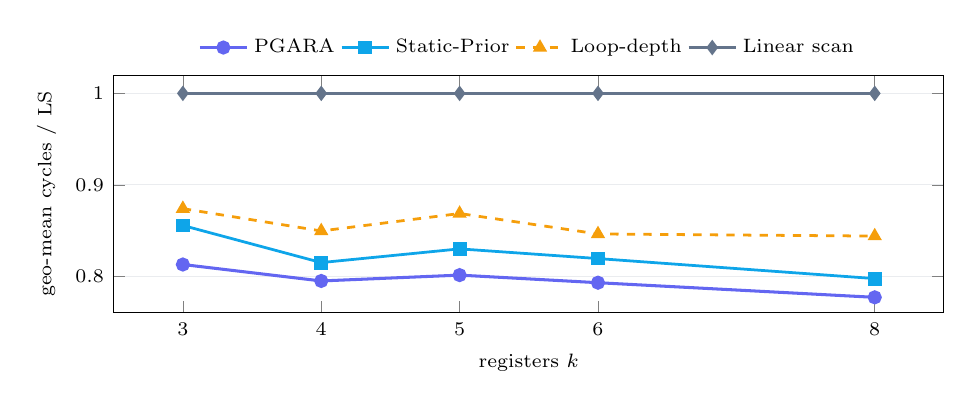
\begin{tikzpicture}
\begin{axis}[
  width=\columnwidth, height=46mm, xlabel={registers $k$},
  ylabel={geo-mean cycles / LS}, xtick={3,4,5,6,8},
  ymin=0.76, ymax=1.02, legend style={font=\scriptsize, at={(0.5,1.03)}, anchor=south, legend columns=4, draw=none},
  tick label style={font=\scriptsize}, label style={font=\scriptsize},
  ymajorgrids, grid style={draw=rule!80}]
\addplot[cPG, mark=*, line width=1.1pt] coordinates {(3,0.8128) (4,0.7948) (5,0.8012) (6,0.7929) (8,0.7769)};
\addplot[cSP, mark=square*, line width=1pt] coordinates {(3,0.8555) (4,0.8149) (5,0.8299) (6,0.8193) (8,0.7974)};
\addplot[cLD, dashed, mark=triangle*, mark options={solid}, line width=1pt] coordinates {(3,0.8739) (4,0.8495) (5,0.8686) (6,0.8462) (8,0.8439)};
\addplot[cLS, mark=diamond*, line width=1pt] coordinates {(3,1) (4,1) (5,1) (6,1) (8,1)};
\legend{\MG, Static-Prior, Loop-depth, Linear scan}
\end{axis}
\end{tikzpicture}
\caption{Geometric-mean cycles over the suite, normalised to linear
scan, as the register budget varies.}
\label{fig:ksweep}
\end{figure}

\subsection{Spill traffic and register utilisation}

Dynamic spill traffic (Fig.~\ref{fig:spills}) is where the
expected-gain objective shows most directly, because (\ref{eq:gain})
is precisely the expected spill traffic avoided. Summed over the suite,
\MG\ executes 59\% fewer spill memory operations than linear scan at
$k=4$, 12\% fewer than Static-Prior and 21\% fewer than loop-depth
priority, and at $k=8$ it nearly eliminates spill traffic (4.6k
operations against 27.9k, 72.2k and 213k). Register utilisation
(Fig.~\ref{fig:util}) follows: the mean fraction of operand accesses
served from registers rises from 77\% at $k=3$ to 98\% at $k=8$ for
\MG, against 69\% to 87\% for linear scan. Note that the number of
\emph{static} spilled values can be higher for \MG\ than for loop-depth
priority (191 against 159 at $k=4$): \MG\ deliberately spills many
cold values in order to keep the few hot ones, which is the intended
behaviour of a gain-maximising allocator.

\begin{figure}[t]
\centering
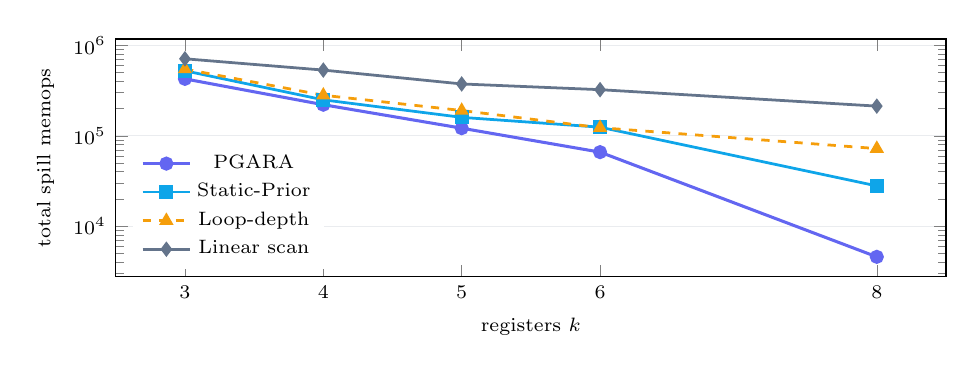
\begin{tikzpicture}
\begin{semilogyaxis}[
  width=\columnwidth, height=46mm, xlabel={registers $k$},
  ylabel={total spill memops}, xtick={3,4,5,6,8},
  legend style={font=\scriptsize, at={(0.02,0.03)}, anchor=south west, draw=none, fill=white},
  tick label style={font=\scriptsize}, label style={font=\scriptsize},
  ymajorgrids, grid style={draw=rule!80}]
\addplot[cPG, mark=*, line width=1.1pt] coordinates {(3,426993) (4,220974) (5,121418) (6,65936) (8,4563)};
\addplot[cSP, mark=square*, line width=1pt] coordinates {(3,525157) (4,250236) (5,160099) (6,124588) (8,27861)};
\addplot[cLD, dashed, mark=triangle*, mark options={solid}, line width=1pt] coordinates {(3,548327) (4,281272) (5,190539) (6,122987) (8,72155)};
\addplot[cLS, mark=diamond*, line width=1pt] coordinates {(3,713119) (4,534475) (5,375411) (6,324336) (8,213194)};
\legend{\MG, Static-Prior, Loop-depth, Linear scan}
\end{semilogyaxis}
\end{tikzpicture}
\caption{Dynamic spill loads and stores summed over the suite
(log scale).}
\label{fig:spills}
\end{figure}

\begin{figure}[t]
\centering
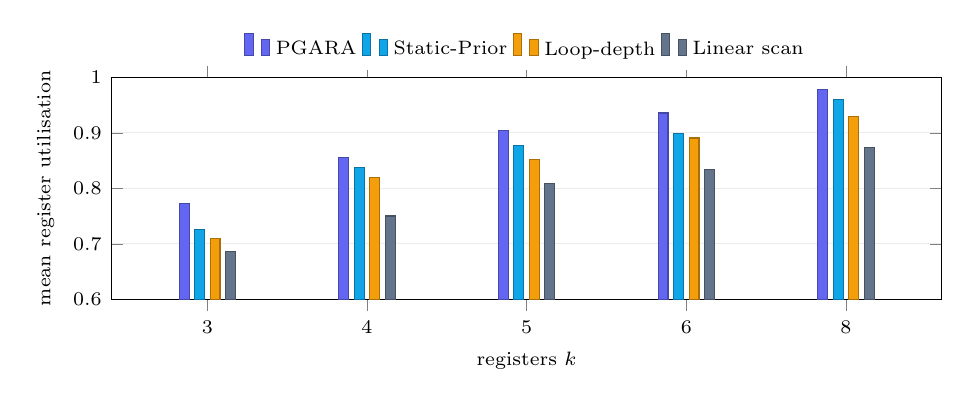
\begin{tikzpicture}
\begin{axis}[
  ybar, bar width=3.6pt, width=\columnwidth, height=44mm,
  xlabel={registers $k$}, ylabel={mean register utilisation},
  symbolic x coords={3,4,5,6,8}, xtick=data, ymin=0.6, ymax=1.0,
  legend style={font=\scriptsize, at={(0.5,1.03)}, anchor=south, legend columns=4, draw=none},
  tick label style={font=\scriptsize}, label style={font=\scriptsize},
  ymajorgrids, grid style={draw=rule!80}, enlarge x limits=0.15]
\addplot[fill=cPG, draw=cPG!70!black] coordinates {(3,0.7722) (4,0.8551) (5,0.9046) (6,0.936) (8,0.9781)};
\addplot[fill=cSP, draw=cSP!70!black] coordinates {(3,0.7252) (4,0.8383) (5,0.8774) (6,0.8982) (8,0.9607)};
\addplot[fill=cLD, draw=cLD!70!black] coordinates {(3,0.7102) (4,0.8199) (5,0.8515) (6,0.8909) (8,0.9293)};
\addplot[fill=cLS, draw=cLS!70!black] coordinates {(3,0.6863) (4,0.7502) (5,0.8082) (6,0.8344) (8,0.8732)};
\legend{\MG, Static-Prior, Loop-depth, Linear scan}
\end{axis}
\end{tikzpicture}
\caption{Mean register utilisation (fraction of operand accesses
served from registers) over the suite.}
\label{fig:util}
\end{figure}

\subsection{Code size and compile cost}

Table~\ref{tab:size} gives static code size summed over the suite.
The three auction-based allocators produce code of similar size,
9--17\% smaller than linear scan, because shared web slots and register
hints remove most $\varphi$ copies, and fewer spilled operands need
explicit loads and stores. Code size is not the objective of \MG, and
Static-Prior is marginally smaller at $k=4$--6. Compile cost is low
(Table~\ref{tab:bench}): policy iteration needs 1.26 improvement rounds
on average over all values and configurations, with a maximum of seven,
and running all four allocators on the largest program (dispatch, 116 SSA values) takes
about 22\,ms in pure Python. Every interference graph in the study was
verified chordal, with the largest clique at 15 values.

\begin{table}[t]
\centering
\caption{Static code size (instructions) summed over the suite}
\label{tab:size}
\footnotesize
\begin{tabular}{@{}lrrrr@{}}
\toprule
$k$ & \MG & Static-Prior & Loop-depth & Linear scan \\
\midrule
3 & \textbf{1486} & 1496 & 1511 & 1661 \\
4 & 1443 & \textbf{1433} & 1439 & 1604 \\
5 & 1395 & \textbf{1385} & 1392 & 1573 \\
6 & 1351 & \textbf{1341} & 1360 & 1541 \\
8 & \textbf{1257} & 1260 & 1297 & 1520 \\
\bottomrule
\end{tabular}
\end{table}

\subsection{Sensitivity to the training input}

A profile-driven allocator is only as good as its profile. Table~\ref{tab:sens}
repeats the three most data-dependent benchmarks at $k=4$ with a
deliberately unrepresentative training input: on rare-branch the error
rate in training is 60\% instead of 1\%; on dispatch and scanner the
training input shifts the case mix. With a mismatched profile \MG\
falls behind Static-Prior by 2--10\%, though it remains ahead of
loop-depth priority and linear scan on all three, only narrowly so on
scanner. The training input must
therefore resemble production behaviour, as with any profile-guided
optimisation~\cite{panchenko2019bolt,wagner1994}, and Static-Prior is
the right fallback when no such input exists.

\begin{table}[t]
\centering
\caption{Cycles ($\times10^3$, $k=4$) with representative and
mismatched training inputs}
\label{tab:sens}
\footnotesize
\setlength{\tabcolsep}{3.5pt}
\begin{tabular}{@{}lrrrrr@{}}
\toprule
& \multicolumn{2}{c}{\MG} & & & \\
\cmidrule(lr){2-3}
Benchmark & repr. & mism. & Static & Loop-d. & Lin.\ scan \\
\midrule
rarebranch & \textbf{338.4} & 398.4 & 390.7 & 423.2 & 516.4 \\
dispatch & \textbf{128.1} & 136.7 & 128.6 & 164.6 & 236.4 \\
scanner & \textbf{412.3} & 459.9 & 417.8 & 464.2 & 530.7 \\
\bottomrule
\end{tabular}
\end{table}

\subsection{Comparison with related approaches}

Table~\ref{tab:compare} positions \MG\ against the classical
allocators it was measured against and against the learned allocator
RL4ReAl~\cite{venkatakeerthy2023rl4real}, which we compare
qualitatively because it targets LLVM's back ends.

\begin{table}[t]
\centering
\caption{Qualitative comparison of allocation approaches}
\label{tab:compare}
\footnotesize
\setlength{\tabcolsep}{2.5pt}
\begin{tabular}{@{}p{17mm}p{18mm}p{14mm}p{12mm}p{12mm}@{}}
\toprule
Approach & Decision basis & Uses measured profile & Training & Explainable \\
\midrule
Linear scan~\cite{poletto1999} & interval order & no & none & partly \\
Loop-depth priority~\cite{chow1990} & $10^{d}$ weights & no & none & yes \\
RL4ReAl~\cite{venkatakeerthy2023rl4real} & learned policy & indirectly & heavy & no \\
\MG\ (this work) & expected gain $G(v)$, auction & yes & none & yes (bids) \\
\bottomrule
\end{tabular}
\end{table}

\subsection{Threats to validity}

The benchmarks are small kernels written for this study, and the
threshold $\theta$ was tuned on the same suite (from the candidates
0.1, 0.25 and 0.5). Cycles come from a simulator with a fixed latency
table rather than from hardware, and PG-RISC has no caches, so the
memory cost is a constant. The MDP charges a value for its whole live
range, while the optimal policy may move it between register and memory
inside the range; the code generator does not split live ranges, so
that part of the policy is computed but not realised.

%% =====================================================================
\section{Conclusion and Future Work}
\label{sec:conclusion}

\MG\ allocates registers adaptively, guided by measured profiles, by
expected gain: a per-value Markov decision
process over the live range, solved exactly with measured branch
probabilities, followed by a sealed-bid auction among $\varphi$-web
coalitions on the chordal SSA interference graph and best-response
dynamics to a Nash equilibrium. Existing allocators either rank values
by static weights that cannot see data-dependent branches or learn
opaque policies from large corpora.

The method makes the expected saving of each decision an explicit
number, needs no training, and costs milliseconds. It is embedded in a
complete compiler, from an LL(1) grammar and attribute-grammar semantic
analysis through TAC, SSA and optimisation to PG-RISC code and a
simulator, with a web interface that shows every phase.

On ten benchmarks and five register budgets, all 200 compiled programs
match the reference output. At $k=4$, \MG\ reduces geometric-mean
cycles by 20.5\% relative to linear scan, 6.4\% relative to loop-depth
priority and 2.5\% relative to static priors, and executes 59\% fewer
spill memory operations than linear scan, with the largest benefits on
programs with skewed, data-dependent control flow.

Future work will extend the MDP's policy into live-range splitting in
the code generator so that values can move between register and memory
inside a range, replace whole-program averages with context-sensitive
or phase-aware profiles to address the cases where the profile
misleads, port the engine to a production back end such as LLVM to
evaluate it on standard suites and real hardware, and combine measured
profiles with learned profile prediction~\cite{rotem2021pgo} when no
representative input is available.

%% =====================================================================
\section*{Author Contributions}

\begin{enumerate}
\item \textbf{Shreyans Chowdry} (24BDS0114): core pipeline design,
lexical and syntax analysis, AST construction and intermediate code
generation.
\item \textbf{Samrender Singh Saini} (24BCE2865): semantic analysis,
scope resolution and symbol table management.
\item \textbf{Karthikeya Jami} (24BCE2136): code optimisation engine
and target assembly and machine code generation.
\item \textbf{Abhishek Kumar} (24BCE0585): runtime environment, test
suite and benchmarking.
\item \textbf{Nishanth Kumar} (24BAI0194): web GUI, pipeline
visualisation interface and documentation.
\end{enumerate}
All authors contributed to the design of the \MG\ allocator and to
the writing of this manuscript.

\section*{Acknowledgements}
The authors thank their course faculty for guidance on recasting the
allocator around stochastic dynamic programming and game theory.

\section*{Funding}
This work received no external funding.

\section*{Competing Interests}
The authors declare no competing interests.

\section*{Data and Code Availability}
The compiler, the web interface, the benchmark programs and the raw
results (JSON and CSV for all 200 configurations and the sensitivity
study) are available from the authors on request.

%% =====================================================================
\begin{thebibliography}{99}
\footnotesize

\bibitem{lattner2021mlir}
C.~Lattner, M.~Amini, U.~Bondhugula, A.~Cohen, A.~Davis, J.~Pienaar,
R.~Riddle, T.~Shpeisman, N.~Vasilache, and O.~Zinenko, ``MLIR: Scaling
compiler infrastructure for domain specific computation,'' in
\emph{Proc.\ IEEE/ACM Int.\ Symp.\ Code Generation and Optimization
(CGO)}, 2021, pp.~2--14.

\bibitem{wang2018ml}
Z.~Wang and M.~O'Boyle, ``Machine learning in compiler optimization,''
\emph{Proc.\ IEEE}, vol.~106, no.~11, pp.~1879--1901, 2018.

\bibitem{ashouri2018survey}
A.~H. Ashouri, W.~Killian, J.~Cavazos, G.~Palermo, and C.~Silvano, ``A
survey on compiler autotuning using machine learning,'' \emph{ACM
Comput.\ Surv.}, vol.~51, no.~5, art.~96, 2018.

\bibitem{leather2020ml}
H.~Leather and C.~Cummins, ``Machine learning in compilers: Past,
present and future,'' in \emph{Proc.\ Forum for Specification and
Design Languages (FDL)}, 2020.

\bibitem{cytron1991ssa}
R.~Cytron, J.~Ferrante, B.~K. Rosen, M.~N. Wegman, and F.~K. Zadeck,
``Efficiently computing static single assignment form and the control
dependence graph,'' \emph{ACM Trans.\ Program.\ Lang.\ Syst.}, vol.~13,
no.~4, pp.~451--490, 1991.

\bibitem{rastello2022ssa}
F.~Rastello and F.~Bouchez~Tichadou, Eds., \emph{SSA-based Compiler
Design}. Cham, Switzerland: Springer, 2022.

\bibitem{cooper2022eac}
K.~D. Cooper and L.~Torczon, \emph{Engineering a Compiler}, 3rd~ed.
Cambridge, MA, USA: Morgan Kaufmann, 2022.

\bibitem{aho2006dragon}
A.~V. Aho, M.~S. Lam, R.~Sethi, and J.~D. Ullman, \emph{Compilers:
Principles, Techniques, and Tools}, 2nd~ed. Boston, MA, USA:
Addison-Wesley, 2006.

\bibitem{chaitin1982}
G.~J. Chaitin, ``Register allocation \& spilling via graph coloring,''
in \emph{Proc.\ SIGPLAN Symp.\ Compiler Construction}, 1982,
pp.~98--105.

\bibitem{chow1990}
F.~C. Chow and J.~L. Hennessy, ``The priority-based coloring approach
to register allocation,'' \emph{ACM Trans.\ Program.\ Lang.\ Syst.},
vol.~12, no.~4, pp.~501--536, 1990.

\bibitem{poletto1999}
M.~Poletto and V.~Sarkar, ``Linear scan register allocation,''
\emph{ACM Trans.\ Program.\ Lang.\ Syst.}, vol.~21, no.~5,
pp.~895--913, 1999.

\bibitem{hack2006ssa}
S.~Hack, D.~Grund, and G.~Goos, ``Register allocation for programs in
SSA-form,'' in \emph{Proc.\ Int.\ Conf.\ Compiler Construction (CC)},
LNCS~3923, 2006, pp.~247--262.

\bibitem{hack2006ipl}
S.~Hack and G.~Goos, ``Optimal register allocation for SSA-form
programs in polynomial time,'' \emph{Inf.\ Process.\ Lett.}, vol.~98,
no.~4, pp.~150--155, 2006.

\bibitem{lozano2019toplas}
R.~Castañeda Lozano, M.~Carlsson, G.~Hjort Blindell, and C.~Schulte,
``Combinatorial register allocation and instruction scheduling,''
\emph{ACM Trans.\ Program.\ Lang.\ Syst.}, vol.~41, no.~3, art.~17,
2019.

\bibitem{lozano2019survey}
R.~Castañeda Lozano and C.~Schulte, ``Survey on combinatorial register
allocation and instruction scheduling,'' \emph{ACM Comput.\ Surv.},
vol.~52, no.~3, art.~62, 2019.

\bibitem{trofin2021mlgo}
M.~Trofin, Y.~Qian, E.~Brevdo, Z.~Lin, K.~Choromanski, and D.~Li,
``MLGO: A machine learning guided compiler optimizations framework,''
arXiv:2101.04808, 2021.

\bibitem{venkatakeerthy2023rl4real}
S.~VenkataKeerthy, S.~Jain, A.~Kundu, R.~Aggarwal, A.~Cohen, and
R.~Upadrasta, ``RL4ReAl: Reinforcement learning for register
allocation,'' in \emph{Proc.\ ACM SIGPLAN Int.\ Conf.\ Compiler
Construction (CC)}, 2023, pp.~133--144.

\bibitem{venkatakeerthy2020ir2vec}
S.~VenkataKeerthy, R.~Aggarwal, S.~Jain, M.~S. Desarkar, R.~Upadrasta,
and Y.~N. Srikant, ``IR2Vec: LLVM IR based scalable program
embeddings,'' \emph{ACM Trans.\ Archit.\ Code Optim.}, vol.~17, no.~4,
art.~32, 2020.

\bibitem{cummins2022compilergym}
C.~Cummins, B.~Wasti, J.~Guo, B.~Cui, J.~Ansel, S.~Gomez, S.~Jain,
J.~Liu, O.~Teytaud, B.~Steiner, Y.~Tian, and H.~Leather, ``CompilerGym:
Robust, performant compiler optimization environments for AI
research,'' in \emph{Proc.\ IEEE/ACM Int.\ Symp.\ Code Generation and
Optimization (CGO)}, 2022, pp.~92--105.

\bibitem{cummins2021programl}
C.~Cummins, Z.~V. Fisches, T.~Ben-Nun, T.~Hoefler, M.~F.~P. O'Boyle,
and H.~Leather, ``ProGraML: A graph-based program representation for
data flow analysis and compiler optimizations,'' in \emph{Proc.\ Int.\
Conf.\ Machine Learning (ICML)}, PMLR~139, 2021, pp.~2244--2253.

\bibitem{panchenko2019bolt}
M.~Panchenko, R.~Auler, B.~Nell, and G.~Ottoni, ``BOLT: A practical
binary optimizer for data centers and beyond,'' in \emph{Proc.\
IEEE/ACM Int.\ Symp.\ Code Generation and Optimization (CGO)}, 2019,
pp.~2--14.

\bibitem{shen2023propeller}
H.~Shen, K.~Pszeniczny, R.~Lavaee, S.~Kumar, S.~Tallam, and X.~D. Li,
``Propeller: A profile guided, relinking optimizer for warehouse-scale
applications,'' in \emph{Proc.\ ACM Int.\ Conf.\ Architectural Support
for Programming Languages and Operating Systems (ASPLOS)}, 2023.

\bibitem{rotem2021pgo}
N.~Rotem and C.~Cummins, ``Profile guided optimization without
profiles: A machine learning approach,'' arXiv:2112.14679, 2021.

\bibitem{wagner1994}
T.~A. Wagner, V.~Maverick, S.~L. Graham, and M.~A. Harrison,
``Accurate static estimators for program optimization,'' in
\emph{Proc.\ ACM SIGPLAN Conf.\ Programming Language Design and
Implementation (PLDI)}, 1994, pp.~85--96.

\bibitem{wu1994}
Y.~Wu and J.~R. Larus, ``Static branch frequency and program profile
analysis,'' in \emph{Proc.\ 27th Annu.\ Int.\ Symp.\ Microarchitecture
(MICRO)}, 1994, pp.~1--11.

\bibitem{sutton2018rl}
R.~S. Sutton and A.~G. Barto, \emph{Reinforcement Learning: An
Introduction}, 2nd~ed. Cambridge, MA, USA: MIT Press, 2018.

\bibitem{puterman1994}
M.~L. Puterman, \emph{Markov Decision Processes: Discrete Stochastic
Dynamic Programming}. New York, NY, USA: Wiley, 1994.

\bibitem{bertsekas2019}
D.~P. Bertsekas, \emph{Reinforcement Learning and Optimal Control}.
Belmont, MA, USA: Athena Scientific, 2019.

\bibitem{howard1960}
R.~A. Howard, \emph{Dynamic Programming and Markov Processes}.
Cambridge, MA, USA: MIT Press, 1960.

\bibitem{bellman1957}
R.~Bellman, \emph{Dynamic Programming}. Princeton, NJ, USA: Princeton
Univ.\ Press, 1957.

\bibitem{shapley1953}
L.~S. Shapley, ``A value for $n$-person games,'' in \emph{Contributions
to the Theory of Games II}, Annals of Mathematics Studies~28.
Princeton, NJ, USA: Princeton Univ.\ Press, 1953, pp.~307--317.

\bibitem{vickrey1961}
W.~Vickrey, ``Counterspeculation, auctions, and competitive sealed
tenders,'' \emph{J.~Finance}, vol.~16, no.~1, pp.~8--37, 1961.

\bibitem{tarjan1984}
R.~E. Tarjan and M.~Yannakakis, ``Simple linear-time algorithms to test
chordality of graphs, test acyclicity of hypergraphs, and selectively
reduce acyclic hypergraphs,'' \emph{SIAM J.\ Comput.}, vol.~13, no.~3,
pp.~566--579, 1984.

\bibitem{rosenthal1973}
R.~W. Rosenthal, ``A class of games possessing pure-strategy Nash
equilibria,'' \emph{Int.\ J.\ Game Theory}, vol.~2, no.~1, pp.~65--67,
1973.

\bibitem{nisan2007agt}
N.~Nisan, T.~Roughgarden, {\'E}.~Tardos, and V.~V. Vazirani, Eds.,
\emph{Algorithmic Game Theory}. Cambridge, U.K.: Cambridge Univ.\
Press, 2007.

\bibitem{jain2022posetrl}
S.~Jain, Y.~Andaluri, S.~VenkataKeerthy, and R.~Upadrasta, ``POSET-RL:
Phase ordering for optimizing size and execution time using
reinforcement learning,'' in \emph{Proc.\ IEEE Int.\ Symp.\ Performance
Analysis of Systems and Software (ISPASS)}, 2022, pp.~121--131.

\bibitem{hajali2020neurovectorizer}
A.~Haj-Ali, N.~K. Ahmed, T.~Willke, Y.~S. Shao, K.~Asanovic, and
I.~Stoica, ``NeuroVectorizer: End-to-end vectorization with deep
reinforcement learning,'' in \emph{Proc.\ IEEE/ACM Int.\ Symp.\ Code
Generation and Optimization (CGO)}, 2020, pp.~242--255.

\bibitem{cummins2023llm}
C.~Cummins, V.~Seeker, D.~Grubisic, M.~Elhoushi, Y.~Liang,
B.~Rozi{\`e}re, J.~Gehring, F.~Gloeckle, K.~Hazelwood, G.~Synnaeve, and
H.~Leather, ``Large language models for compiler optimization,''
arXiv:2309.07062, 2023.

\bibitem{knuth1965lr}
D.~E. Knuth, ``On the translation of languages from left to right,''
\emph{Inf.\ Control}, vol.~8, no.~6, pp.~607--639, 1965.

\bibitem{lewis1968}
P.~M. Lewis and R.~E. Stearns, ``Syntax-directed transduction,''
\emph{J.~ACM}, vol.~15, no.~3, pp.~465--488, 1968.

\bibitem{knuth1968attr}
D.~E. Knuth, ``Semantics of context-free languages,'' \emph{Math.\
Syst.\ Theory}, vol.~2, no.~2, pp.~127--145, 1968.

\bibitem{cooper2001dom}
K.~D. Cooper, T.~J. Harvey, and K.~Kennedy, ``A simple, fast dominance
algorithm,'' Rice Univ., Houston, TX, USA, Tech.\ Rep., 2001.

\bibitem{wegman1991sccp}
M.~N. Wegman and F.~K. Zadeck, ``Constant propagation with conditional
branches,'' \emph{ACM Trans.\ Program.\ Lang.\ Syst.}, vol.~13, no.~2,
pp.~181--210, 1991.

\bibitem{python}
Python Software Foundation, ``Python 3 documentation,'' 2024.
[Online]. Available: \url{https://docs.python.org/3/}

\bibitem{playwright}
Microsoft, ``Playwright: Fast and reliable end-to-end testing for
modern web apps,'' 2024. [Online]. Available:
\url{https://playwright.dev/}

\end{thebibliography}

\end{document}
